% Chapter 4
\chapter{Implementação}
\label{Capítulo4}

\begin{center}
	\textit{``Do or do not. There is no try.''}

	Master Yoda
\end{center}
Este capítulo aprofunda os aspectos técnicos do LaRE, tomando como referência a arquitetura apresentada na Figura \ref{fig:arquitecturalore}.

O desenvolvimento começou pela implementação e desenvolvimento do servidor \textit{Flask} e página \textit{web}, sendo que o primeiro circuito a ser implementado e testado foi a Lei de Ohm. O projecto foi evoluindo com a adição dos restantes circuitos que compõem o \acrshort{lare}.

Para o desenvolvimento do \textit{software}, utilizou-se o \acrshort{ide} \textit{Visual Studio Code}\footnote{\url{https://code.visualstudio.com/}}, e o projeto encontra-se alojado no \textit{GitHub}. O sistema operativo instalado no \gls{RaspberryPI} é uma versão ligeiramente modificada do \textit{Arch Linux ARM}.

Os circuitos que compõem o \acrshort{lare} foram testados e validados individualmente em placas brancas, antes de se proceder à construção da matriz de placas, como referido na Secção \ref{sec:matriz}.

No Anexo \ref{AppendixA} - \textit{datasheet} - encontram-se todos os esquemas completos das experiências, assim como as placas que constituem a matriz do \acrshort{lare}: cada uma ficou dividida por uma placa, mais uma dedicada às fontes de alimentação, num total de três placas. 

\section{Hardware}
\subsection{Registo de deslocamento}
\label{sec:hwregistodeslocamento}
O \textit{SN74HC595} é um registo de deslocamento de 8 \textit{bits} do tipo \acrshort{sipo}, cujo funcionamento já foi detalhado na Secção \ref{sec:registodeslocamento}. Uma trama de (até 8) \textit{bits} é enviada pelo \gls{RaspberryPI} para o registo através do pino \acrshort{ser}. Na Figura \ref{fig:esquematico74hc595} pode ver-se o diagrama explicativo do processo de envio:

\begin{enumerate}
	\item Pinos \acrshort{oe} e \acrshort{srclr} activados;
	\item Um \textit{bit} ``0'' ou ``1'' é enviado para o pino \acrshort{ser};
	\item \textit{N} impulsos ascendentes no pino \acrshort{srclk} fazem com que o \textit{N bits} sejam enviado para o registo de deslocamento (\textit{N bits} <= 8);
	\item Um impulso ascendente no pino \acrshort{rclk} faz com que os \textit{N bits} sejam enviados para o registo de memória e, por conseguinte, para os relés (através do \textit{ULN2003A}).
\end{enumerate}

%Por cada impulso ascendente no pino \textit{SRCLK} - \textit{Shift Register Clock} - Os \textit{bits} são enviados um-a-um para o registo de deslocamento. No final, um impulso ascendente no \textit{RCLK} - \textit{Register Clock} - faz com que os \textit{bits} sejam enviados para o registo de memória e, por conseguinte, para os relés.

\begin{figure}[hbtp]
	\centering
	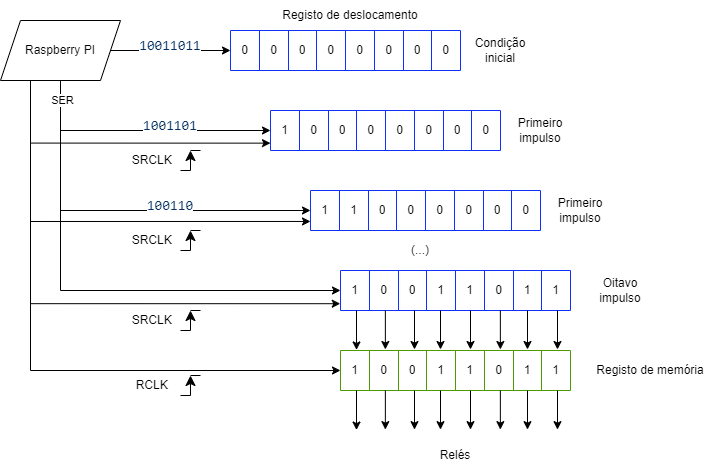
\includegraphics[width=0.7\textwidth]{figures/registo deslocamente.drawio.png}
	\caption{Envio de \textit{bits} para o registo de deslocamento}
	\label{fig:esquematico74hc595}
\end{figure}

\subsection{Driver de relés}
\label{sec:driverreles}
Conforme referido na Secção \ref{sec:driver}, o \gls{RaspberryPI} não tem capacidade para comandar os relés. Para esse efeito, é necessário utilizar um \textit{driver} de relés. A Figura \ref{fig:diagramablocos2003} apresenta o diagrama simplificado para uma entrada/saída do \textit{driver} \cite{ULN2003}.

\begin{figure}[hbtp]
	\centering
	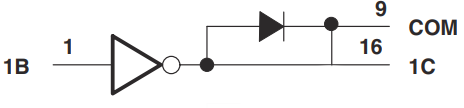
\includegraphics[width=0.4\textwidth]{figures/uln2003_diagramablocos.png}
	\caption{Diagrama de blocos simplificado do \textit{ULN2003A}}
	\label{fig:diagramablocos2003}
\end{figure}

O terminal 9 - \textit{COM} - é ligado à tensão de comando dos relés e é destinado aos díodos de ``roda livre'', conforme mencionado na Secção \ref{sec:reles}. No caso dos modelos de relés utilizados neste projecto, a tensão é de \SI{12}{\volt}. Se o valor lógico na entrada ``1B'' = ``0'' (ou \SI{0}{\volt}), então, a saída ``1C'' = ``1'' (ou \SI{12}{\volt}) - 
O \textit{ULN2003A} faz parte da família dos \textit{drivers} inversores.

As Figuras \ref{fig:comandorelesfull} e \ref{fig:exemplovoltimetro} servem como exemplos práctico que ilustram o funcionamento do procedimento referido na Figura \ref{fig:esquematico74hc595}. Neste exemplo, foi utilizado um relé \acrshort{spst}. No entanto, o funcionamento é idêntico para os relés \acrshort{dpst}, variando apenas a disposição dos pinos.

\begin{figure}[hbtp]
	\centering%
		\centering
		\subfloat[\centering Ligação \textit{SN74HC595} - \textit{ULN2003A}\label{fig:comandorelesfull}]{{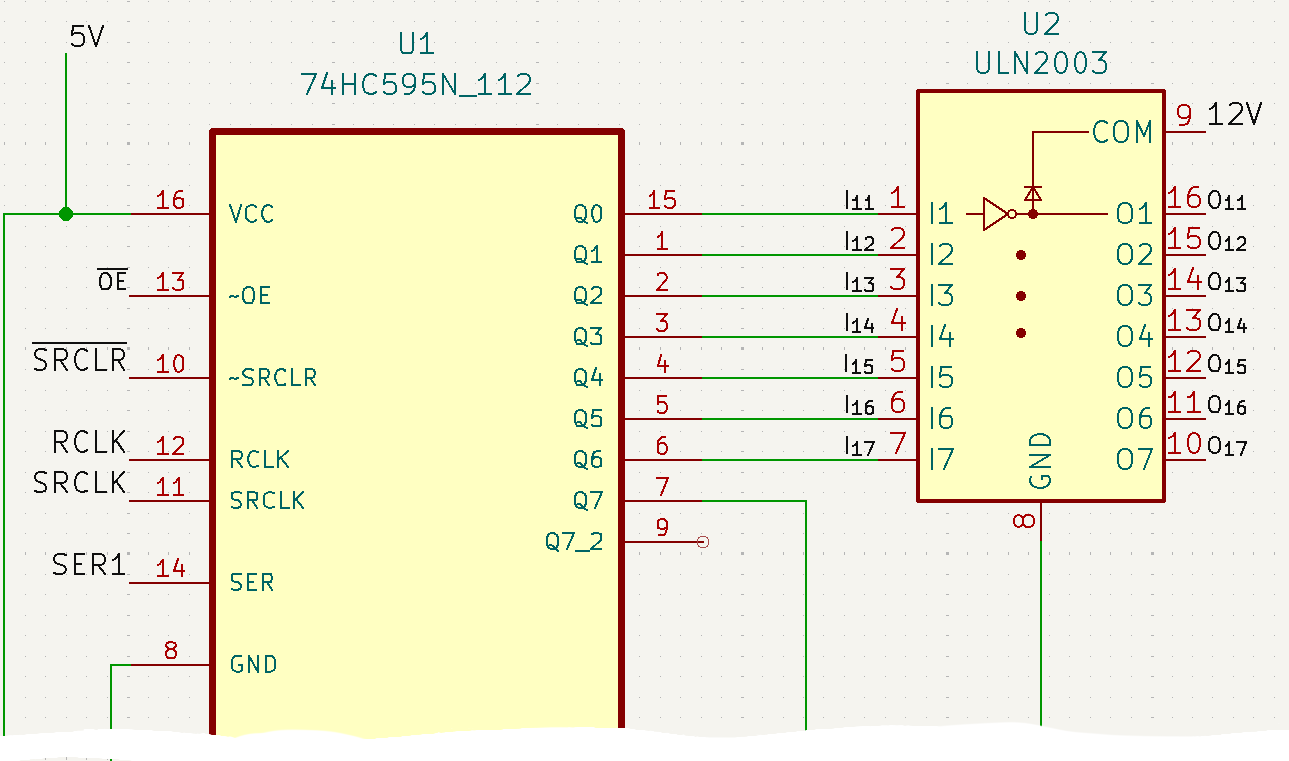
\includegraphics[width=6cm]{figures/comandoreles_FULL.png} }}%
		\qquad
		\subfloat[\centering Exemplo comando do voltímetro\label{fig:exemplovoltimetro}]{{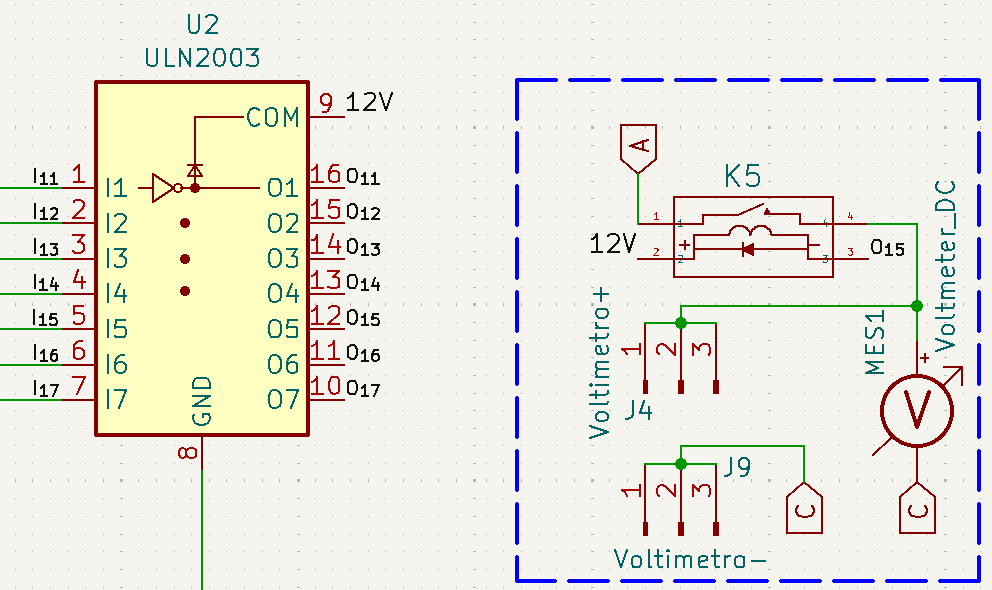
\includegraphics[width=6cm]{figures/exemplo_voltimetro.png} }}%
		\caption{Exemplo de uso do \textit{SN74HC595} e \textit{ULN2003A}}%
		\label{fig:ligacao5952003}%
	\end{figure}

As entradas $I_{1}$ a $I_{7}$ recebem os \textit{bits} enviados pelo \gls{RaspberryPI} através do registo de deslocamento, conforme apresentado na Figura \ref{fig:comandorelesfull}. As saídas $O_{1}$ a $O_{7}$ controlam os relés nos terminais ``3'', enquanto os terminais ``2'' dos relés são ligados aos \SI{12}{\volt}, como ilustrado na Figura \ref{fig:exemplovoltimetro}.
%O funcionamento está descrito na Listagem \ref{Table:exemplouln2003}:

% \begin{table}[htb]
% 	\centering
% 	\caption{Tabela funcionamento \textit{ULN2003A} e relés}
% 	\label{Table:exemplouln2003}
% 	\begin{tabular}{ccc}
% 		\toprule
% 		\multicolumn{2}{c}{ULN2003A} & Relés                                \\
% 		\midrule
% 		Entrada                      & Saída                  & Estado      \\
% 		\midrule
% 		``0'' (\SI{0}{\volt})        & ``1'' (\SI{12}{\volt}) & Desactivado \\
% 		\midrule
% 		``1'' (\SI{12}{\volt})       & ``0'' (\SI{0}{\volt})  & Activado    \\
% 		\bottomrule
% 	\end{tabular}
% \end{table}

No caso particular do exemplo descrito em cima, se $I_{5} = I_{15}$ = \SI{0}{\volt}, então, a saída $O_{5}$ = \SI{12}{\volt} e não há diferença nos terminais ``2'' e ``3'' na bobina do relé  ``K5''. O relé está desactivado. Por outro lado, se $I_{5} = I_{15}$ = \SI{12}{\volt}, então, a saída $O_{5}$ = \SI{0}{\volt}, há diferença de potencial aos terminais da bobina e o relé está activado.

No caso em que a trama a ser transmitida for maior que 8 \textit{bits}, há a necessidade de usar mais do que um registo de deslocamento. Neste caso, o pino 9 - $Q_{H}'$ - do primeiro registo é ligado ao pino \acrshort{ser} do segundo registo e assim sucessivamente.

\subsection{Relés}
\label{sec:hwreles}
Como já foi referido na Secção \ref{sec:solucaoproposta}, o \acrshort{lare} é composto por cinco circuitos. A implementação começou com o desenho esquemático e, tal como referido na Secção \ref{sec:reles}, tentou-se, sempre que possível, utilizar os relés \acrshort{spst} no comando das fontes e aparelhos de medida e os relés \acrshort{dpst} no controlo dos componentes, tal como se pode ver na Figura \ref{fig:relespstdpst}. O relé \textit{K4} - \acrshort{spst} - comanda a fonte de alimentação de \SI{5}{\volt} e os relés \textit{K1} a \textit{K3} - \acrshort{dpst} - comandam os componentes.

\begin{figure}[hbtp]
	\centering
	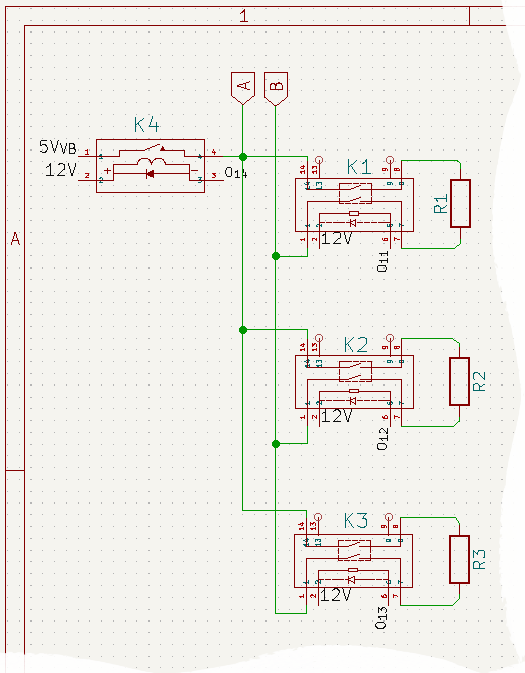
\includegraphics[width=0.3\textwidth]{figures/exemplo_reles_spst.png}
	\caption{Exemplo de utilização de relés \acrshort{spst} e \acrshort{dpst}}
	\label{fig:relespstdpst}
\end{figure}

\subsection{Fontes de alimentação}
\label{sec:fontesalimentacao}

O \acrshort{lare} utiliza várias fontes de alimentação, todas passíveis de serem controladas por \textit{software} e neste aspecto tentou-se simplificar/limitar o uso de fontes externas, além das que poderiam ser fornecidas pelo \acrshort{virtualbench}. 

Como pode ser visto na Figura \ref{fig:paineldianteiro} ou na Figura \ref{fig:promenorfontes} com mais pormenor, o \acrshort{virtualbench} possuí três fontes de alimentação (\acrshort{cc} variáveis): \SI{+6}{\volt}, \SI{+25}{\volt} e \SI{-25}{\volt}\footnote{No contexto do \acrshort{lare} a fonte de tensão negativa não é usada.}.

\begin{figure}[hbtp]
	\centering
	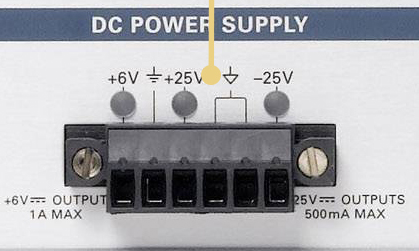
\includegraphics[width=0.5\textwidth]{figures/fontes_VB.png}
	\caption{Fontes de tensão do \acrshort{virtualbench}}
	\label{fig:promenorfontes}
\end{figure}

Assim, o \acrshort{lare} utiliza os seguintes níveis de tensão/fontes de alimentação:
\begin{itemize}
	\item \SI{1}{\volt} - \SI{5}{\volt} variáveis (\acrshort{cc}), utilizadas na experiência da Lei de Ohm;
	\item \SI{12}{\volt} (\acrshort{cc}) - utilizada na alimentação dos relés e dos \textit{drivers};
	\item \SI{5}{\volt} (\acrshort{cc}) - utilizada na alimentação do registo de deslocamento;
	\item Para o estudo dos circuitos rectificadores e filtros utilizou-se um transformador \SI{220}{\volt}/\SI{8}{\volt} \acrshort{ca}.
\end{itemize}

\subsubsection{Fonte de tensão \SI{6}{\volt} - variável e {Fonte de tensão \SI{12}{\volt} - fixa}}
\label{sec:fontes6-12}
As fontes de tensão de \SI{6}{\volt}, utilizadas na Lei de \textit{Ohm} e de \SI{12}{\volt}, destinadas à alimentação dos relés e dos \textit{drivers}, são fornecidas diretamente pelo \acrshort{virtualbench}. As configurações são definidas por \textit{software} e podem ser consultadas na Secção \ref{sec:configmedicaoes}.

\begin{figure}[hbtp]
	\centering%
		\centering
		\subfloat[\centering Introdução\label{fig:schfonte5VB}]{{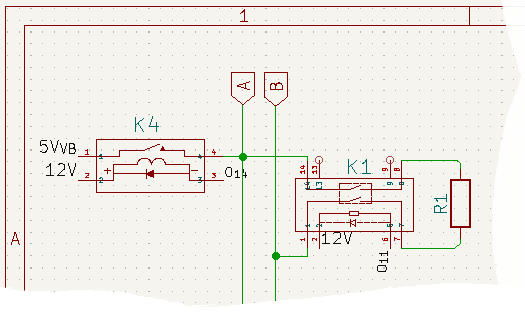
\includegraphics[width=6cm]{figures/sch_fonte5VB.png} }}%
		\qquad
		\subfloat[\centering Controlo\label{fig:schfonte12VB}]{{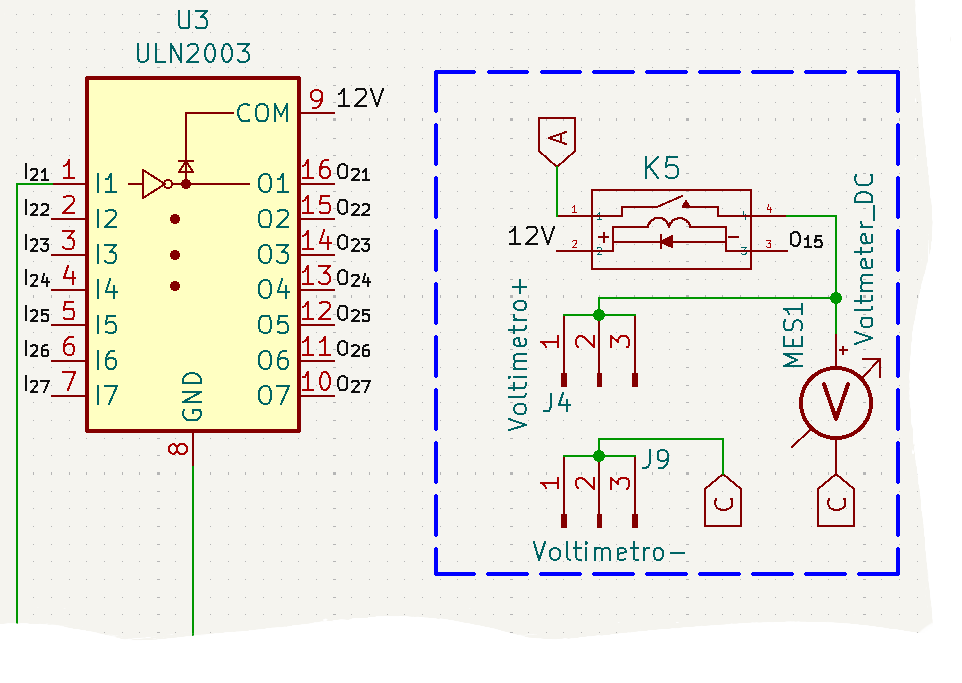
\includegraphics[width=6cm]{figures/sch_fonte12V.png} }}%
		\caption{Implementação Fontes de \SI{6}{\volt} e \SI{12}{\volt}}%
		\label{fig:fontes6-12}%
	\end{figure}

As Figuras \ref{fig:schfonte5VB} e \ref{fig:schfonte12VB} ilustram os exemplos das ligações das respetivas fontes de tensão. Complementando com a Figura \ref{fig:promenorfontes}, o terminal 4 do relé $K_{4}$, designado por $5V_{VB}$, está ligado ao terminal de \SI{6}{\volt} do \acrshort{virtualbench}, enquanto todos os terminais 2 dos relés, assim como a alimentação dos \textit{drivers}, estão ligados ao terminal de \SI{25}{\volt}. As configurações destes valores são definidas por \textit{software} e podem ser consultadas na Secção \ref{sec:configmedicaoes}.

\subsubsection{Fonte de tensão \SI{5}{\volt} - fixa}
De forma a alimentar os circuitos com \SI{5}{\volt} fixos foi projectada - Figura \ref{fig:esqlm317} e implementada - Figura \ref{fig:impllm317} - uma fonte de alimentação \cite{LM317}.

\begin{figure}[hbtp]
	\centering%
		\centering
		\subfloat[\centering Esquemático\label{fig:esqlm317}]{{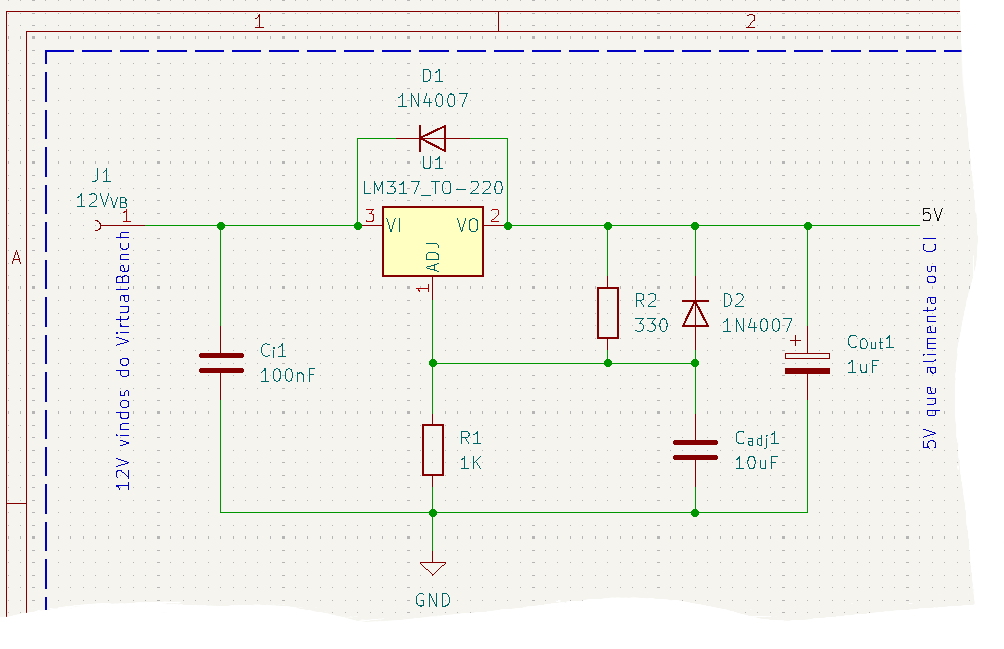
\includegraphics[width=6.3cm]{figures/sch_fonte5V.png} }}%
		\qquad
		\subfloat[\centering Implementação\label{fig:impllm317}]{{\includegraphics[width=6.3cm]{figures/fonte_LM317.png} }}%
		\caption{Fonte de \SI{5}{\volt} \textins{LM317}}%
		\label{fig:fonte5V}%
	\end{figure}

Esta fonte teve como base o LM317 e o esquema presente na página 11, Figura 9, do \textit{datasheet} \cite{LM317}. A utilização do LM317 em detrimento, por exemplo, do LM7805 prendeu-se com a disponibilidade do regulador em contexto laboratorial. Este regulador serve perfeitamente os propósitos deste projecto, já que a tensão de saída, regulável, varia entre os \SI{1.25}{\volt} e os \SI{37}{\volt} e a corrente de saída pode ser superior a \SI{1.5}{\ampere}. 

Relativamente aos díodos de protecção, $D_{1}$ e $D_{2}$, representados no esquema da Figura \ref{fig:fonte5V}, em vez de se usarem os díodos 1N4002, por uma questão de disponibilidade dos componentes, usaram-se os díodos 1N4007. Estes díodos pertencem à mesma família de diodos retificadores da série 1N400x. Ambos têm especificações elétricas e mecânicas semelhantes, nomeadamente, a capacidade de suportar correntes directas até \SI{1}{\ampere} - valor suficiente para o nosso projecto que, relembre-se, é limitado pelo \acrshort{virtualbench} a \SI{0.5}{\ampere}. No entanto, a principal diferença entre eles está na tensão inversa máxima que cada modelo é capaz de suportar \cite{1N400x}:

\begin{itemize}
	\item 1N4002: Possui uma tensão inversa máxima de 100 V;
	\item 1N4007: Suporta uma tensão inversa máxima de 1000 V.
\end{itemize}

Estes valores são, pois, mais que suficientes para os níveis de tensão usados.

Sendo assim, para uma tensão de saída de \SI{5}{\volt}, calcularam-se as resistências com base na expressão apresentada do \textit{datasheet}, representada na Equação \ref{eq:calculolm317}: 

\begin{equation} \label{eq:calculolm317}
	V_{O} = V_{REF} (1 + \frac{R_{2}}{R_{1}}) + (I_{ADJ} \times R_{2})
\end{equation}

De notar que, segundo o \textit{datasheet} do LM317 \cite{LM317}, $V_{REF} = \SI{1.25}{\volt}$ e o valor do termo $I_{ADJ} \times R_{2}$ pode ser simplificado. De facto, $I_{ADJ}$ é, tipicamente, \SI{50}{\micro\ampere}, sendo que, para o nosso projecto, o valor escolhido para $R_{2}$ foi de \SI{1}{\kilo\ohm}. Assim, segundo a Equação \ref{eq:simplificação}, tem-se que:
\begin{equation} \label{eq:simplificação}
	V_{ADJ} = I_{ADJ} \times R_{2} = \SI{0.05}{\volt}
\end{equation}

A Equação \ref{eq:calculolm317} fica então reduzida a:

\begin{equation} \label{eq:calculoR1simplificado}
	V_{O} = V_{REF} (1 + \frac{R_{2}}{R_{1}})
\end{equation}

Considerando $V_{O} = \SI{5}{\volt}$, e uma vez que a Equação \ref{eq:calculoR1simplificado} tem duas incógnitas, $R_{1}$ e $R_{2}$, atribuiu-se a $R_{2}$ o valor de \SI{1}{\kilo\ohm}, tal como foi dito anteriormente. Desta forma, obteve-se $R_{1} = \SI{333.33(3)}{\ohm}$, tal como descrito na Equação \ref{eq:calculoR1}: 

\begin{equation} \label{eq:calculoR1}
	\SI{5}{\volt} = 1.25 \times (1 + \frac{1000}{R_{1}}) \Leftrightarrow R_{1} = \SI{333.33(3)}{\ohm}
\end{equation}

O valor da resistência normalizada mais próxima é de \SI{330}{\ohm}. Importa, pois, reverter a Equação \ref{eq:calculoR1simplificado} e confirmar o valor de  $V_{O}$ obtido:

\begin{equation} \label{eq:confirmacaoVout}
	V_{O} = 1.25 \times (1 + \frac{1000}{330}) \Leftrightarrow V_{O} = \SI{5,037(87)}{\volt}
\end{equation}

Portanto, este é um valor perfeitamente aceitável para alimentar os circuitos integrados.

\subsubsection{Fontes de tensão \SI{220}{\volt}/\SI{8}{\volt} CA}
\label{sec:fontealternada}
As experiências respeitantes aos rectificadores e filtros utilizam tensão alternada sinusoidal. Tal como já foi referido anteriormente, tentou-se, sempre que possível, simplificar o uso de fontes externas. 

Na prática e em contexto de sala de aula, a experiência de rectificação de onda completa levanta um problema de massas, se se pretender usar um gerador de sinal. Quer isto dizer que não é possível medir, simultaneamente, os sinais de entrada e saída. Como se pode ver pelo esquema representado na Figura \ref{fig:gerador-massa}, o díodo está curto-circuitado (linha magenta a tracejado, entre os pontos 2 e 3) devido ao facto das massas serem comuns. 

\begin{figure}[hbtp]
	\centering
	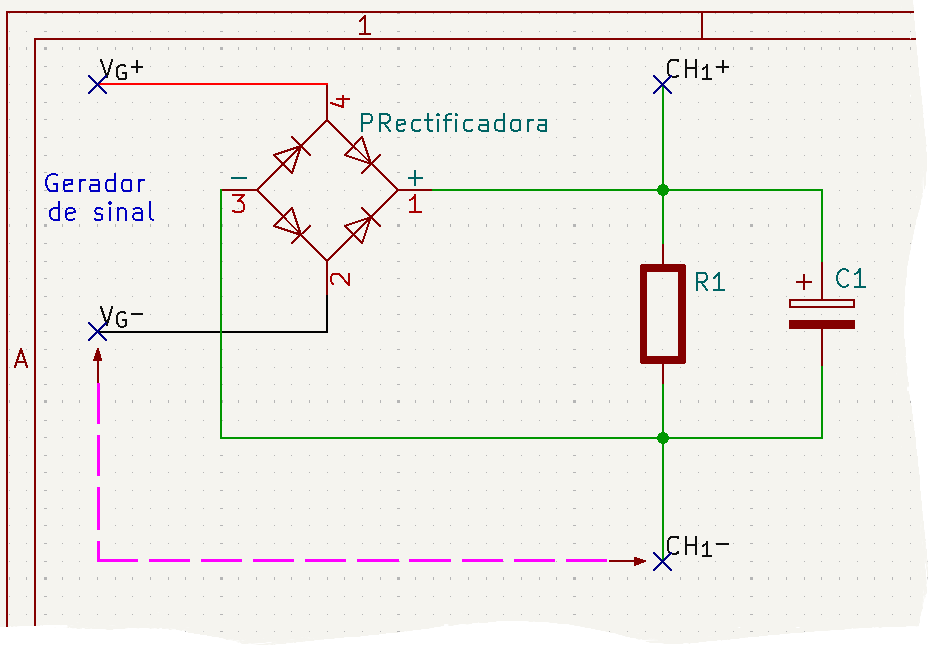
\includegraphics[width=0.5\textwidth]{figures/sch_completa_CC.png}
	\caption{Problema de massa - onda completa}
	\label{fig:gerador-massa}
\end{figure}

A forma de contornar este problema é usar um transformador e, assim, medir a onda de saída com o osciloscópio, tal como representado no esquema da Figura \ref{fig:ondacompleta-massa}. Ainda assim, não é possível medir as ondas de entrada e saída \textbf{simultaneamente}, se for esse o objectivo.

No caso do \acrshort{lare}, e com recurso ao uso de relés, é possível controlar as massas por \textit{software} e representar as duas ondas na mesma imagem.
De referir que, desta forma, seria possível usar o gerador de sinal. No entanto, o uso do transformador justifica-se pelas seguintes razões:
\begin{itemize}
	\item Facilidade e simplicidade em controlar as massas por \textit{software} - três no caso do uso do gerador de sinal ($CH_{1-}$, $CH_{2-}$ e $VG_{-}$) ou duas no caso de se usar um transformador ($CH_{1-}$, $CH_{2-}$);
	\item Em contexto laboratorial e de sala de aula usa-se um transformador para rectificar a onda completa.
\end{itemize}

%No entanto, para o estudo da rectificação da onda completa, tal não foi possível. Enquanto que no rectificador de meia-onda (... e filtros) é possível usar o gerador de sinal do \acrshort{virtualbench} para medir as ondas de entrada e saída simultaneamente, tal não é possível na rectificação de onda completa, devido ao problema das massas e consequente curto-circuito do díodo na ponte rectificadora. 
%Este problema está representado na Figura \ref{fig:ondacompleta-massa}

\begin{figure}[hbtp]
	\centering
	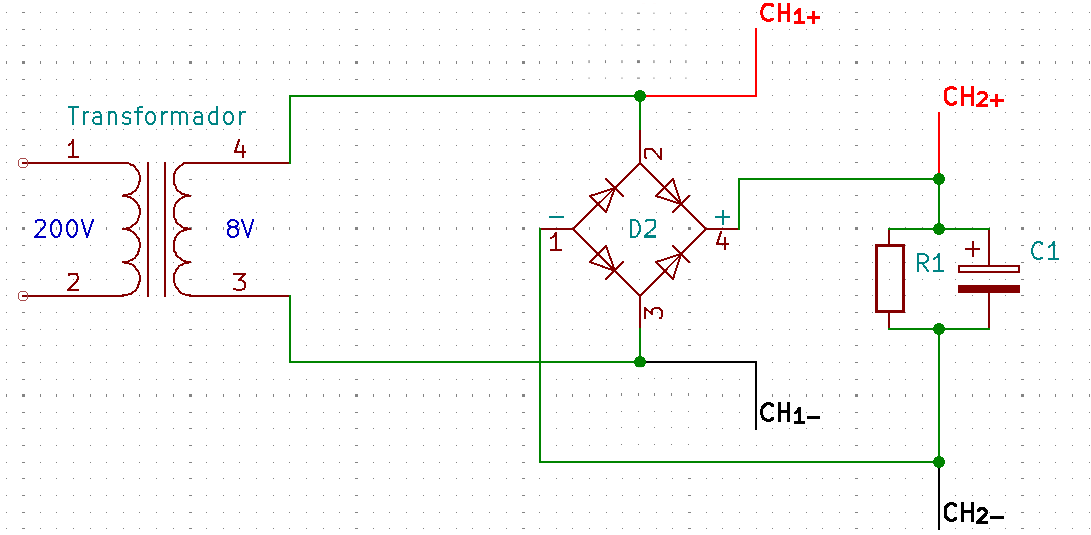
\includegraphics[width=0.7\textwidth]{figures/sch-ondacompleta-massa.png}
	\caption{Problema de massa - onda completa}
	\label{fig:ondacompleta-massa}
\end{figure}

O esquema completo da experiência de rectificação de onda completa pode ser consultado no Anexo~\ref{AppendixA}.

%$CH_{1-}$ e $CH_{2-}$ são as massas do gerador de sinal e osciloscópio (dois canais), respectivamente. É fácil perceber que estando ligados ao mesmo aparelho de medida, neste caso o \acrshort{virtualbench}, as massas dos dois canais do osciloscópio são comuns e, por isso, entre os pontos 2 e 3, o díodo está curto-circuitado. 


%No que concerne à fonte de alimentação \acrshort{ca}, esta foi implementada de forma independente do \acrshort{virtualbench}. \textbf{Falar sobre a fonte de alimentação variável e a fonte de alimentação \acrshort{ca}. Colocar a foto do esquema e explicar como se faz a rectificação, cálculos inclusive. Talvez referir o facto de que depende da qualidade e valores dos transformadores e depois concluir com os valores deste caso, pode-se referir que relativamente à fonte AC, só está disponível a fonte do gerador de sinal do VB e é mais fácil controlar através da fonte externa projectada.}

\subsection{Aparelhos de medida - voltímetro e amperímetro}
\label{sec:aparelhosmedida}

A medição de tensão e corrente são feitas utilizando o multímetro digital - \Acrfull{dmm} - PXI-4072, referenciado na Secção \ref{sec:visir}, Figura \ref{fig:PXI-4072} e cujo painel frontal está representado na Figura \ref{fig:frontDMM}.

\begin{figure}[hbtp]
	\centering
	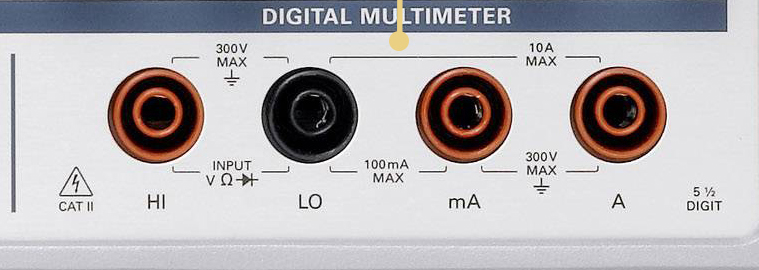
\includegraphics[width=0.5\textwidth]{figures/promenorDMM.png}
	\caption{Painel frontal Multímetro Digital}
	\label{fig:frontDMM}
\end{figure}

Na Figura \ref{fig:esq_geral_ohm} está representado o esquema simplificado da Lei de \textit{Ohm} que pode ilustrar o funcionamento dos aparelhos de medida. O ponto C é comum e é controlado pelo relé $K_{7}$. O terminal positivo do voltímetro está ligado ao ponto A, controlado pelo relé $K_{5}$ mas o amperímetro necessita de mais um relé, já que o controlo da medição é diferente. Neste caso o relé $K_{8}$ funciona como um \textit{bypass} quando se pretende medir tensão e o relé $K{6}$ controla o terminal positivo do amperímetro. 

\begin{figure}[hbtp]
	\centering%
		\centering
		\subfloat[\centering Esquema implementado\label{fig:esq_geral_ohm}]{{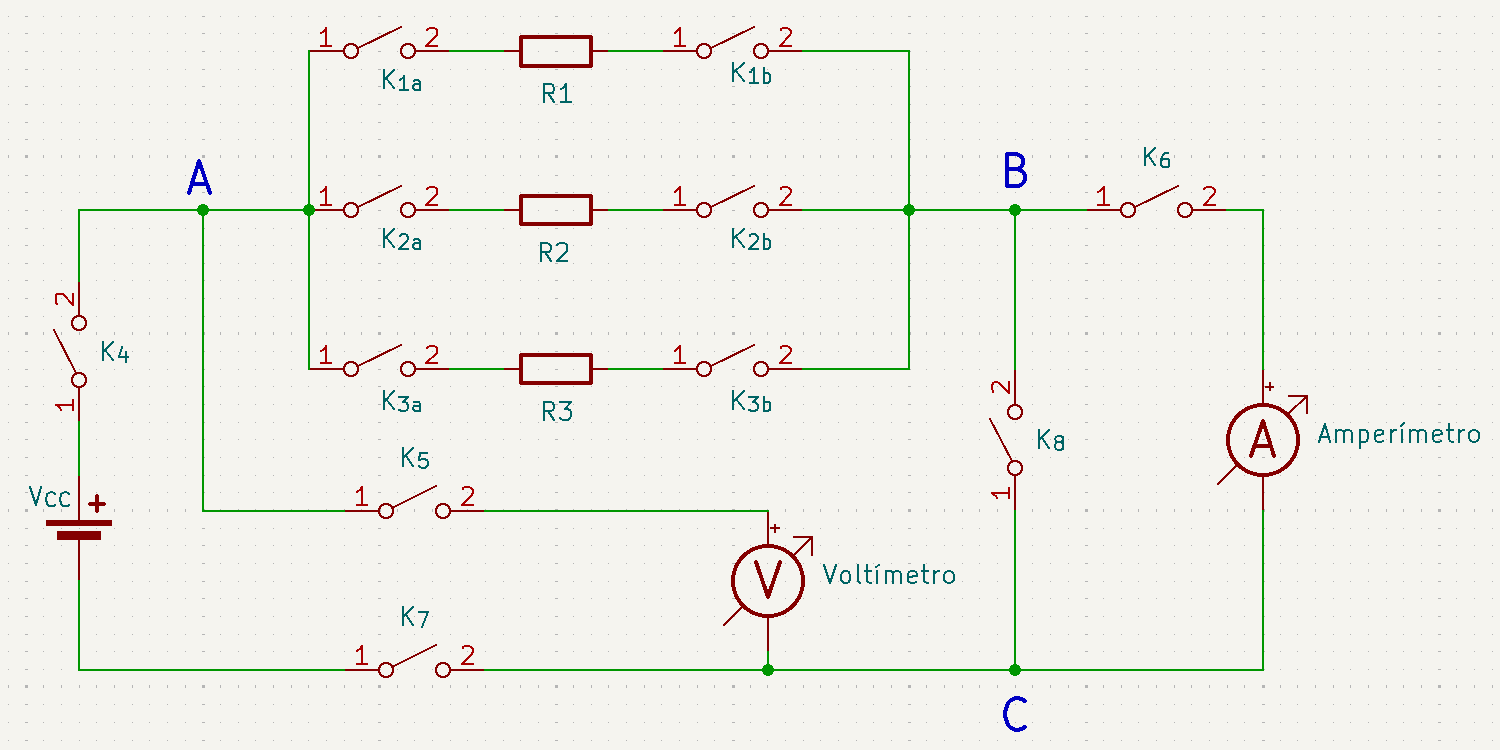
\includegraphics[width=6.3cm]{figures/esquema_simplificado_OHM.png} }}%
		\qquad
		\subfloat[\centering Esquema com os relés duplos\label{fig:full_reles}]{{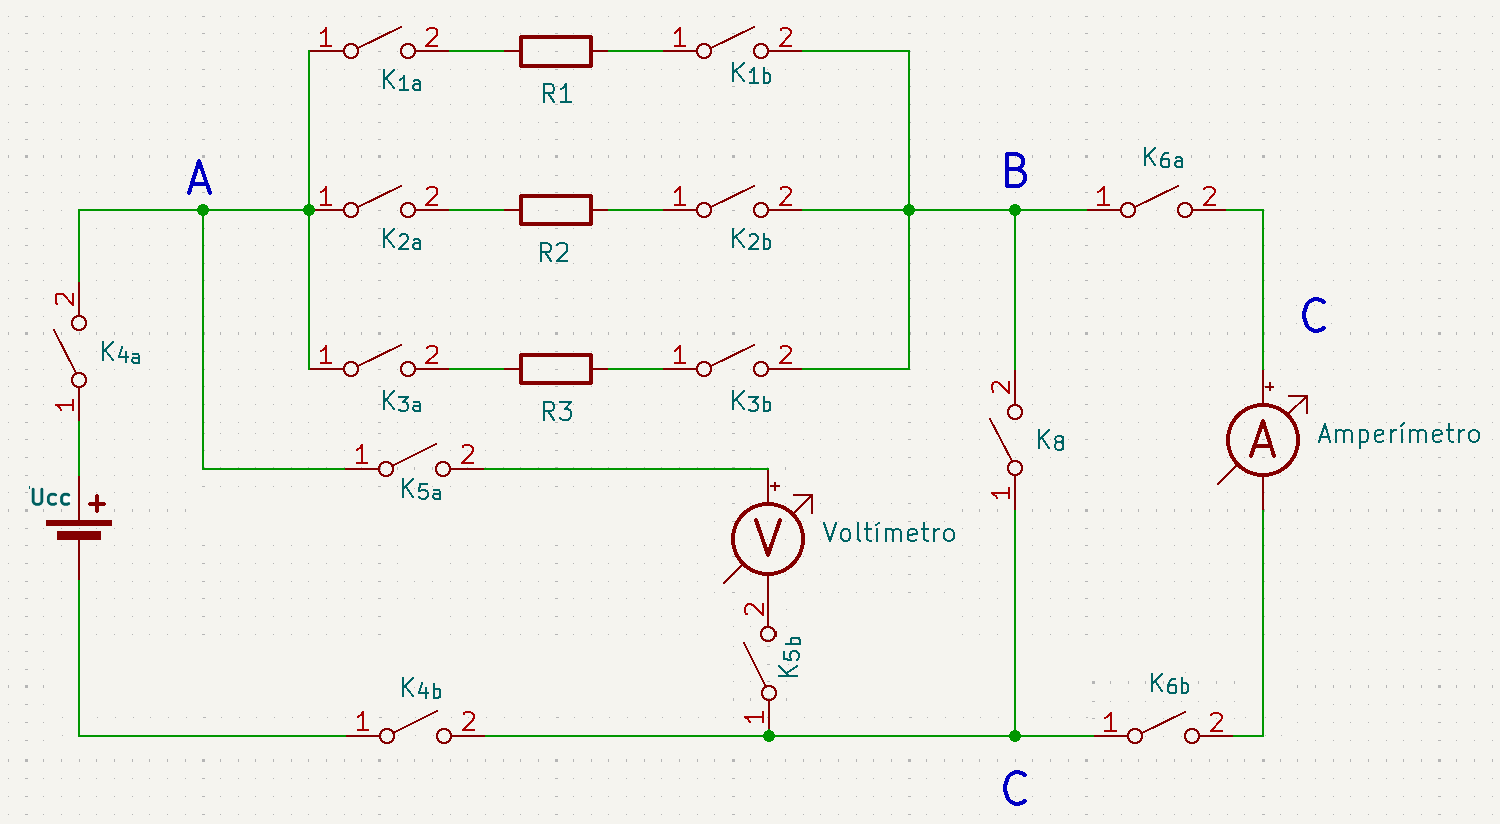
\includegraphics[width=6.3cm]{figures/esquema_simplificado_OHM_IDEAL.png} }}%
		\caption{Esquema completo - Lei de \textit{Ohm}}%
		\label{fig:}%
	\end{figure}

No entanto, faz-se notar o seguinte: Embora os aparelhos de medida sejam independentes, partilham a mesma massa. Esta escolha foi motivada pela indisponibilidade de relés duplos em contexto laboratorial, pelo que se optou por fazer a gestão da forma a que o propósito do projecto fosse atingido e o conceito provado. Na Figura \ref{fig:full_reles} apresenta-se o esquema simplificado, com os relés duplos, adicionados aos aparelhos de medida. 

De referir que, se se pretender expandir o \acrshort{lare} com mais circuitos, é possível utilizar o voltímetro e o amperímetro da forma como estão implementados. 
%Tal como pode ser visto na o voltímetro está disponível entre os pontos A e C e o amperímetro entre os pontos B e C.

A Tabela \ref{Table:exemplomedicaoohm} apresenta o estado dos relés, $K_{5}$ a $K_{8}$ consoante a grandeza que se pretende medir.

\subsection{Experiências}
\label{sec:experiencias}
Nesta secção e seguintes, considera-se, com excepção da Lei de \textit{Ohm}, que cada experiência compreende dois circuitos, isto é, a experiência da rectificação compreende o circuito de meia onda e onda completa; a experiência dos filtros compreende o circuito passa-baixo e passa-alto.

De forma a permitir um melhor desenvolvimento, foco, organização, detecção e correcção de erros, as experiências foram implementadas de forma independente. As primeiras ideias passavam por, além da Lei de \textit{Ohm}, implementar o estudo da rectificação de meia e onda completa. Contudo, verificou-se que seria possível incluir uma experiência adicional, dedicada ao estudo prático de filtros passa-alto e passa-baixo, já que estas duas experiências possuem componentes comuns, ampliando, assim, o alcance e a aplicabilidade do \acrshort{lare}.

A matriz é constituída por três placas, cujos detalhes técnicos podem ser consultados no Anexo \ref{AppendixA}. 
O desenho dos esquemas  e dos \acrfull{pcb} das placas foram elaborados com recurso ao \gls{kicad}. Estas foram desenhadas de forma a serem modulares e estão divididas como representado na Figura \ref{fig:matrizlare}:

\begin{figure}[hbtp]
	\centering
	\includegraphics[width=0.4\textwidth]{figures/lare_3placas.png}
	\caption{Matriz do \acrshort{lare}}
	\label{fig:matrizlare}
\end{figure}
\begin{comment}
ESTA JUSTIFICAÇÃO DEVERIA FICAR NOUTRO LADO - VERIFICARq!!!!

	\textbf{NOTA: Colocar aqui uma imagem do lare completo, com vista dos conectores??? ou só os conectorres?}
Na Secção \ref{sec:fontesalimentacao}, foram já descritas todas as fontes de alimentação do \acrshort{lare}. Com base na Figura \ref{fig:rectificacao_filtragem_full}, o gerador de sinal é controlado pelo relé duplo $K_{1}$, enquanto o díodo é isolado através do relé duplo $K_{3}$ (representado pelo rectângulo tracejado a vermelho escuro).

No que respeita ao relé $K_{4}$, este seria, eventualmente, dispensável, uma vez que o terminal negativo do gerador de sinal é igualmente controlado por $K_{1}$. No entanto, considerando que os filtros (identificados pelo rectângulo tracejado a cor-de-laranja) são partilhados com os circuitos rectificadores, e prevendo a possibilidade de utilização do gerador de sinal noutra experiência, optou-se, por uma questão de segurança, pelo isolamento completo dos componentes através do relé $K_{4}$.
\end{comment}

\subsubsection{Objectivos}
\label{sec:objectivosexperiencias}
\paragraph{Lei de \textit{Ohm}}
Na forma da Equação \ref{eq:leideohm}, a Lei de \textit{Ohm} estabelece que a resistência eléctrica ($R$) de um condutor é determinada pelo quociente entre a tensão elétrica ($U$) aplicada aos seus terminais e a corrente eléctrica ($I$) que o atravessa.  

\begin{equation} \label{eq:leideohm}
	R=\dfrac{U}{I}
\end{equation}

Isto significa que a Equação \ref{eq:leideohm} define uma relação linear entre a tensão e a corrente para uma determinada resistência de valor fixo, o que implica que o gráfico obtido, representado na Figura \ref{fig:graphohm}, é uma linha recta que passa pela origem. O declive dessa recta representa o valor da resistência elétrica ($R$).

\begin{figure}[hbtp]
	\centering
	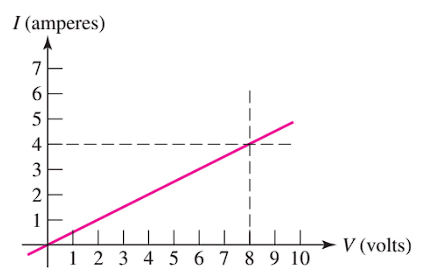
\includegraphics[width=0.3\textwidth]{figures/grafico_Ohm.png}
	\caption{Gráfico da Lei de \textit{Ohm}}
	\label{fig:graphohm}
\end{figure}

Da forma como foi implementado, há duas possibilidades de realizar este estudo, exemplificado nas Figuras \ref{fig:Opção_1} e \ref{fig:Opção_2}. O tutor ou professor, poderá optar por apresentar o conceito de duas formas distintas, em ambos os casos são efectuadas cinco medições, construido o respectivo gráfico e calculado o valor do declive da recta analiticamente. A diferença está na forma como se confrontam os resultados práticos. No entanto, no contexto desta dissertação foi  implementado o caso descrito na Figura \ref{fig:Opção_1}\footnote{Como trabalho futuro, o menu poderia ser desenvolvido para o utilizador, aluno ou professor escolher a opção pretendida.}. 

\begin{figure}[hbtp]
	\centering%
		\centering
		\subfloat[\centering Opção 1\label{fig:Opção_1}]{{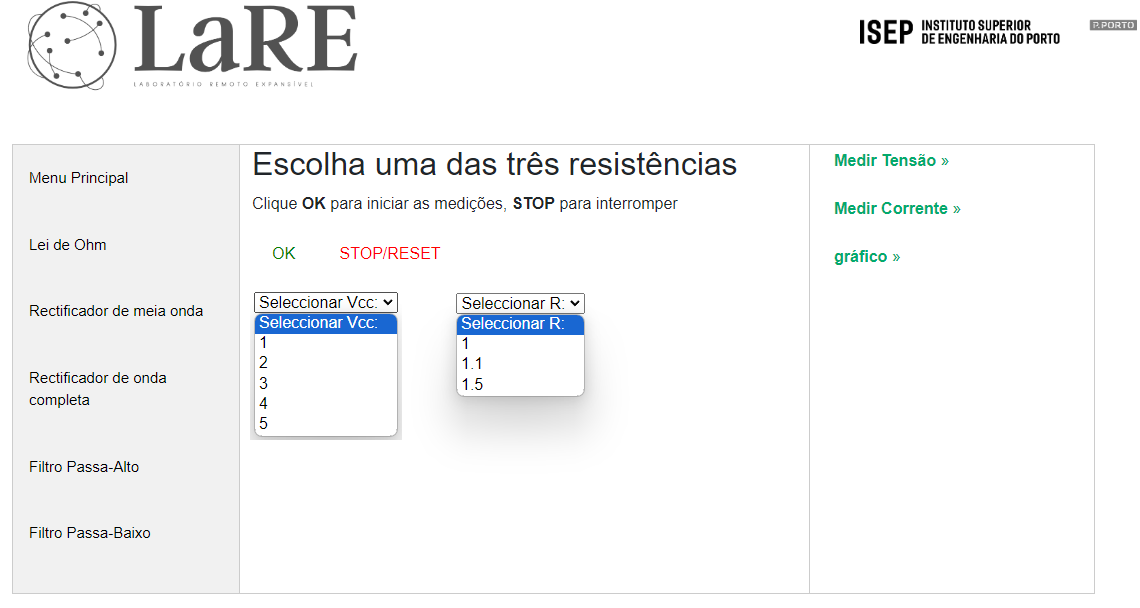
\includegraphics[width=6.3cm]{figures/ohm_escolha.png} }}%
		\qquad
		\subfloat[\centering Opção 2\label{fig:Opção_2}]{{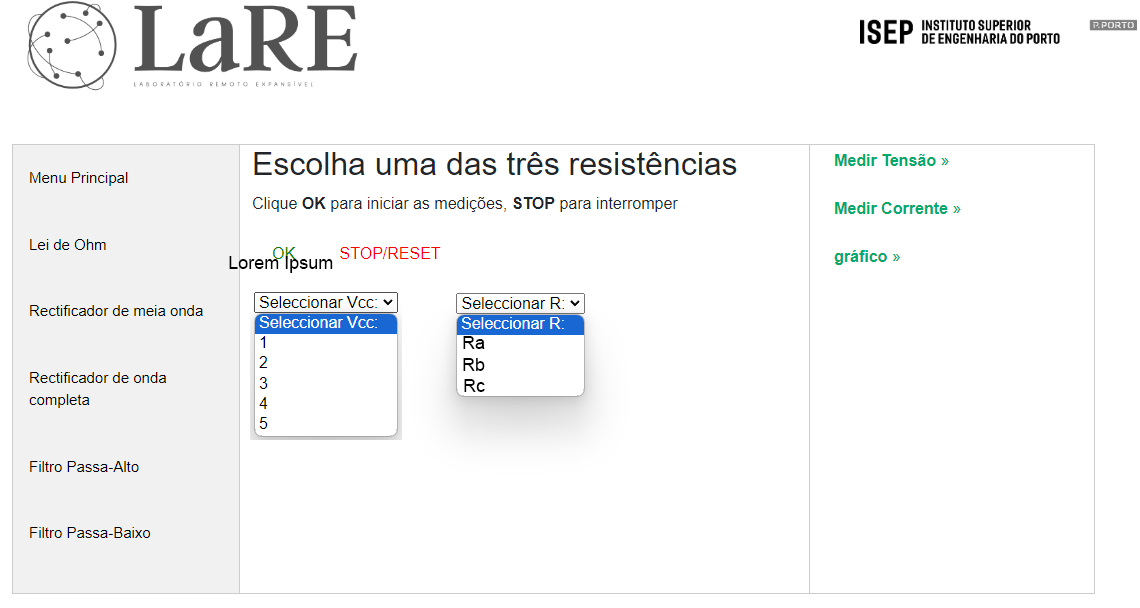
\includegraphics[width=6.3cm]{figures/ohm_escolha_abc.png} }}%
		\caption{Experiência Lei de \textit{Ohm}}%
		\label{fig:experienciaOHM}%
	\end{figure}

No caso em que a resistência é dada, o declive pode ser calculado e confrontado com as soluções, sendo que no caso em que é desconhecida, o declive da recta é calculado e a partir deste do resultado infere-se o valor da resistência. 

\paragraph{Rectificadores}
Nas experiências dos rectificadores pretende-se estudar e avaliar a diferença entre os dois tipos de rectificação, consoante as quatro combinações possíveis dos pares resistência/condensador e a influência que têm na variação da tensão de \textit{ripple}. No caso da rectificação de meia onda, é ainda possível variar a frequência entre os \SI{50}{\hertz} e \SI{2000}{\hertz} mas no caso da rectificação de onda completa, a frequência é fixa ao valor da rede eléctrica - \SI{60}{\hertz}.

A tensão de \textit{ripple} é uma componente variável no tempo que surge à saída do filtro do rectificador, Bloco 3, como representado na Figura \ref{fig:blocosrectificacao}. Esta componente deve ser minimizada para estabilizar a tensão de saída em corrente contínua, Bloco 4, representado na mesma figura \cite{sedrasmith}.

A Figura \ref{fig:sedraripple} representa a forma de onda à saída do Bloco 3 - Filtragem - quando se utiliza a rectificação de meia onda.
\begin{figure}[hbtp]
	\centering
	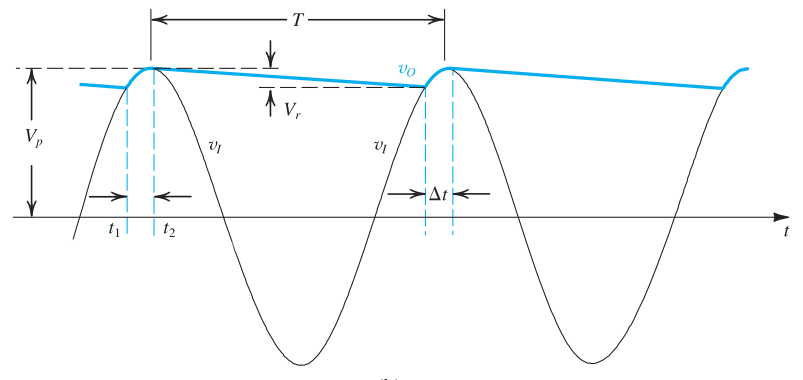
\includegraphics[width=0.7\textwidth]{figures/sedra_ripple.png}
	\caption{Forma de onda à saída do Bloco 3 - Filtragem [meia onda] \cite{sedrasmith}}
	\label{fig:sedraripple}
\end{figure}

A tensão de \textit{ripple} pode ser calculada através da Equação \ref{eq:vripple}:

\begin{equation} \label{eq:vripple}
	U_{r} = \frac{U_{P}}{fRC}
\end{equation}

Observa-se, a partir da Figura \ref{fig:sedraripple} e também da Equação \ref{eq:vripple} que, quando a constante de tempo $CR >> T$, a tensão de \textit{ripple} é pequena. Sendo que, $v_{o}$, ou seja, a tensão à saída do filtro é practicamente constante e dada pela Equação \ref{eq:tensaosaida}:

\begin{equation} \label{eq:tensaosaida}
	u_{o} = U_{P} - \dfrac{1}{2}U_{r}	
\end{equation}

No entanto, pode tornar-se este circuito mais eficiente se se usar a rectificação de onda completa e como pode ser visto na Figura \ref{fig:sedraripplecompleta}, a frequência do \textit{ripple} é o dobro da frequência da onda de entrada.

\begin{figure}[hbtp]
	\centering
	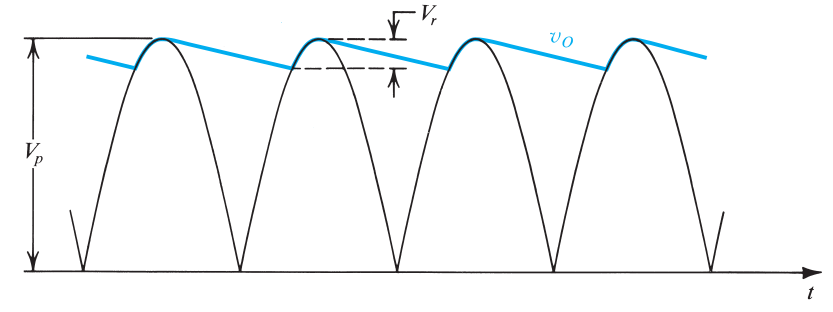
\includegraphics[width=0.7\textwidth]{figures/sedra_ripple_OC.png}
	\caption{Forma de onda à saída do Bloco 3 - Filtragem [onda completa] \cite{sedrasmith}}
	\label{fig:sedraripplecompleta}
\end{figure}

Sendo assim, o valor da tensão de \textit{ripple}, neste caso, será dado pela Equação \ref{eq:vrippleOC}:

\begin{equation} \label{eq:vrippleOC}
	U_{r} = \frac{U_{P}}{2fRC}
\end{equation}

São estas formas de onda, representadas pelas Figuras \ref{fig:sedraripple} e \ref{fig:sedraripplecompleta}, que se pretendem estudar e avaliar, assim como os valores dados pelas Equações \ref{eq:vripple} e \ref{eq:vrippleOC}.

\paragraph{Filtros}
Representados na Figura \ref{fig:filtrosesqgeral} estão os filtros simplificados, leccionados em contexto de sala de aula no ensino secundário.

\begin{figure}[hbtp]
	\centering%
		\centering
		\subfloat[\centering Filtro passa-baixo\label{fig:filtro_pb}]{{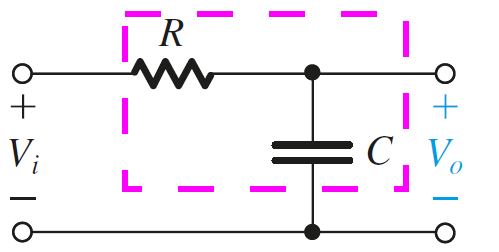
\includegraphics[width=6cm]{figures/Sedra_FPB_GIMP.png} }}%
		\qquad
		\subfloat[\centering Filtro passa-alto\label{fig:filtro_pa}]{{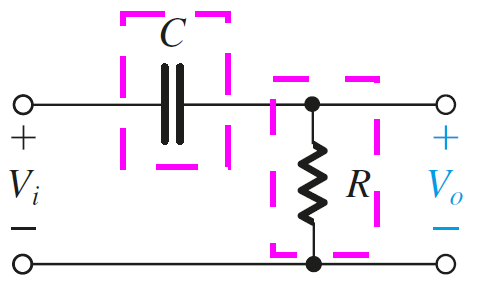
\includegraphics[width=6cm]{figures/Sedra_FPA_GIMP.png} }}%
		\caption{Esquemas dos filtros \cite{sedrasmith}}%
		\label{fig:filtrosesqgeral}%
\end{figure}

A possibilidade de variar a frequência do sinal de entrada permite que estas experiências sejam utilizadas para estudar a resposta em frequência dos filtros, analisar o Diagrama de \textit{Bode}, determinar a frequência de corte dada pela Equação \ref{eq:frequenciacorte} e ainda relacionar, por exemplo, o valor da tensão de entrada com a tensão de saída. 

\begin{equation} \label{eq:frequenciacorte}
	f_{c} = \frac{1}{2\pi RC}
\end{equation}

\begin{comment}
	\textbf{Acho que não é necessário referir a relação entre a tensão de entrada e a tensão de saída, já que isso é feito na parte de software. O que se pode fazer é referir que o \acrshort{lare} permite estudar a resposta em frequência dos filtros, analisar o Diagrama de \textit{Bode} e determinar a frequência de corte.}
A Figura \ref{fig:diagramabode} apresenta um exemplo do Diagrama de \textit{Bode} de um filtro passa-alto, obtido nos testes do LaRE.

\begin{figure}[hbtp]
	\centering
	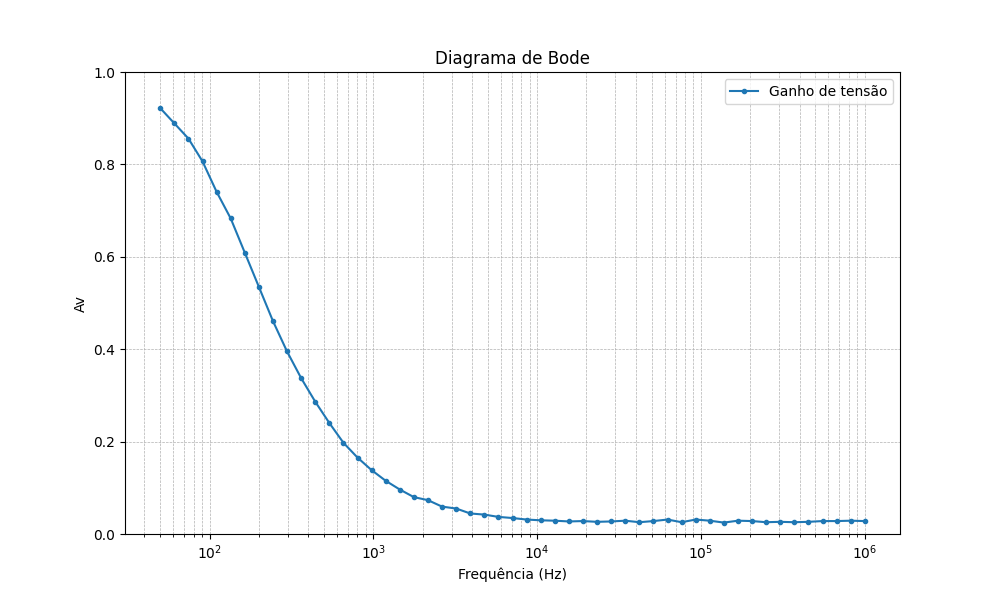
\includegraphics[width=0.6\textwidth]{figures/bode_lpf.png}
	\caption{Diagrama de \textit{Bode} - Filtro passa-alto}
	\label{fig:diagramabode}
\end{figure}
\end{comment}

As Figuras \ref{fig:Bode_pb} e \ref{fig:Bode_pa} apresentam os Diagramas de \textit{Bode} \textins{ideais}, que servem de referência para o estudo desta experiência. 

\begin{figure}[hbtp]
	\centering%
		\centering
		\subfloat[\centering Filtro passa-baixo\label{fig:Bode_pb}]{{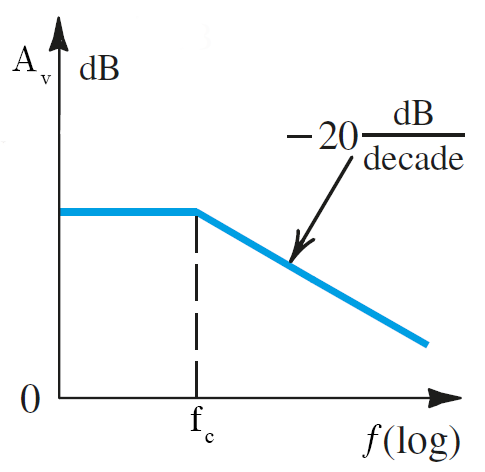
\includegraphics[width=6cm]{figures/Sedra_BodeFPB.png} }}%
		\qquad
		\subfloat[\centering Filtro passa-alto\label{fig:Bode_pa}]{{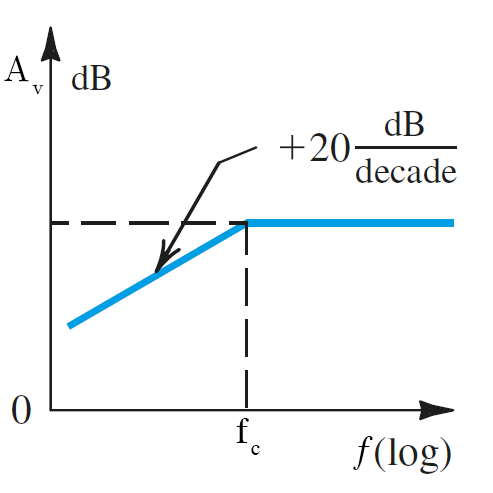
\includegraphics[width=6cm]{figures/Sedra_BodeFPA.png} }}%
		\caption{Diagramas de \textit{Bode} \textins{ideal} \cite{sedrasmith}}%
		\label{fig:Bodeesqgeral}%
\end{figure}

	Para além da análise em frequência, um outro aspeto complementar a considerar é a relação entre as ondas de entrada e saída, em função da frequência. Nos filtros, o intervalo de frequências permitido é igual ao já referido para os rectificadores: entre \SI{50}{\hertz} a \SI{2000}{\hertz}. 
	
	A frequência de corte de um filtro é definida como o ponto onde o ganho do filtro sofre uma atenuação de \SI{3}{\decibel} em relação ao seu valor máximo. 	Para um filtro passa-baixo (passa-alto) ideal, o ganho em baixas (altas) frequências é unitário. Quando o sinal atinge a frequência de corte, a relação entre a tensão de saída e a tensão de entrada reduz-se para:  
	
	\begin{equation} \label{eq:relacaoGanho}
		\frac{U_{out}}{U_{in}} = \frac{1}{\sqrt{2}} \approx 0.707
	\end{equation}
	
	\ldots ou na escala logarítmica:  
\begin{equation} \label{eq:relacaoGanhodB}
	\frac{U_{out}}{U_{in}} = 20 \log_{10} (0.707) \approx -\SI{3}{\decibel}	
\end{equation}
	
Assim, a frequência de corte de um filtro corresponde ao ponto em que a amplitude do sinal de saída é aproximadamente $70.7\%$ da amplitude do sinal de entrada, o que corresponde a -\SI{3}{\decibel}. 

\subsubsection{Lei de Ohm}
\label{sec:lei_ohm}
Na Figura \ref{fig:esq_geral_ohm}, está representado o esquema da Lei de \textit{Ohm} implementado na práctica. A fonte de tensão e os aparelhos de medida foram projetados de forma a serem independentes, tal como referido na Secção \ref{sec:aparelhosmedida}, permitindo a sua utilização caso se pretenda expandir o \acrshort{lare} com mais experiências. A fonte de tensão pode ser utilizada desativando $K_{5}$ e $K7$.

O funcionamento do circuito é relativamente simples, sendo que qualquer que seja a resistência a medir, é fechado o respectivo relé - $K_{1}$ ou $K_{2}$ ou $K_{3}$; a fonte $U_{CC}$ é ligada ao circuito através do relé $K_{4}$ e $K_{7}$.

A medição da tensão e da corrente faz-se da seguinte forma:
\begin{itemize}
	\item Medição da tensão:
	      \begin{itemize}
		      \item Os relés $K_{5}$ e $K_{8}$ são fechados e $K_{6}$ é aberto (Amperímetro desactivado). Desta forma, o voltímetro fica em paralelo com a resistência a medir - entre os pontos A e B.
	      \end{itemize}
	\item Medição da corrente:
	      \begin{itemize}
		      \item Os relés $K_{5}$ e $K_{8}$ são abertos (voltímetro desactivado) e $K_{6}$ é fechado. Desta forma, o amperímetro fica em série com a resistência a medir - entre os pontos B e C.
	      \end{itemize}
\end{itemize}

% Já foi referenciado acima
% Como se pode pode ver na Figura \ref{fig:frontDMM}, retirada da Figura \ref{fig:paineldianteiro}, o terminal negativo (preto) é comum a ambos os aparelhos de medida, que na Figura \ref{fig:esq_geral_ohm} está representado pelo ponto ``C''. O terminal positivo (vermelho) do voltímetro liga ao ponto A - depois de activo o relé $K_{5}$ e o terminal positivo (vermelho) do amperímetro liga ao ponto B - depois de activo o relé $R_{6}$.

Como exemplo, se se pretender estudar a Lei de Ohm para a resistência $R_{1}$, os relés seriam activados da forma representada na Tabela \ref{Table:exemplomedicaoohm}:

\begin{table}[htb]
	\centering
	\caption{Exemplo funcionamento de medição da Lei de Ohm} 
	
	\label{Table:exemplomedicaoohm}
	\begin{tabular}{lcccccccc}
		\toprule
		               & \multicolumn{8}{c}{Estado dos relés}                                                                       \\
		\midrule
		               & $K_{1}$                              & $K_{2}$ & $K_{3}$ & $K_{4}$ & $K_{5}$ & $K_{6}$ & $K_{7}$ & $K_{8}$ \\
		\midrule
		Medir Tensão   & 1                                    & 0       & 0       & 1       & 1       & 0       & 1       & 1       \\
		\midrule
		Medir Corrente & 1                                    & 0       & 0       & 1       & 0       & 1       & 1       & 0       \\
		\bottomrule
	\end{tabular}
\end{table}

\begin{comment}
	% \textbf{Falta o complemento com imagens do gráfico/resultado final e a imagem da placa já feita, opinião PROF}
	Na Figura \ref{fig:esq_geral_ohm} está representado o esquema simplificado do circuito.
Na Figura \ref{fig:graphohm} está representado um exemplo de um gráfico obtido com a experiência da Lei de Ohm, nos testes do \acrshort{lare}.

\begin{figure}[hbtp]
	\centering
	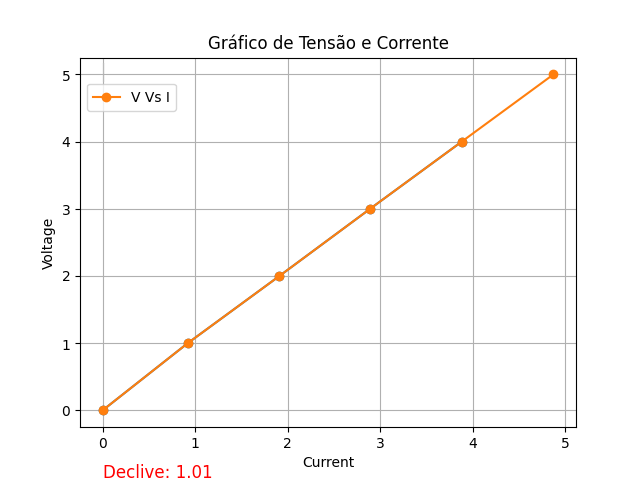
\includegraphics[width=0.6\textwidth]{figures/ohm_graph.png}
	\caption{Exemplo de gráfico Lei de \textit{Ohm}}
	\label{fig:graphohm}
\end{figure}
\end{comment}

A placa desenvolvida para esta experiência, assim como a referência aos ``blocos'', está representada na Figura \ref{fig:placaleideohm}. 

\begin{figure}[hbtp]
	\centering
	\includegraphics[width=0.5\textwidth]{figures/lare_ohm_BLOCOS.png}
	\caption{Implementação práctica da Lei de \textit{Ohm}}
	\label{fig:placaleideohm}
\end{figure}

\begin{enumerate}
	\item Ligação ao \gls{RaspberryPI} através de um conector \acrfull{idc} de 40 pinos (1);
	\item Relés (2);
	\item Ligações aos aparelhos de medida (3);
	\item \textit{Drivers} de relés e registo de deslocamento (4);
	\item Resistências em estudo (5);
	\item Ligação à placa seguinte através de conectores ``Arduino stackable'' (6).
\end{enumerate}

\subsubsection{Rectificadores e filtros}
\label{sec:rectificadoresfiltros}
Uma vez que a implementação destas duas experiência foi realizada na mesma placa, além de que partilham componentes, optou-se por apresentá-las em conjunto. 

Na Figura \ref{fig:rectificacao_filtragem_full} estão representados os esquemas simplificados dos circuitos. Nela se podem ver os componentes comuns - rectângulo tracejado laranja - assim como os rectificadores de meia e onda completa - rectângulo tracejado vermelho e verde, respectivamente. Exclusivo dos filtros estão, também, representados, o condensador e resistência, no rectângulo tracejado magenta.

\begin{figure}[hbtp]
	\centering
	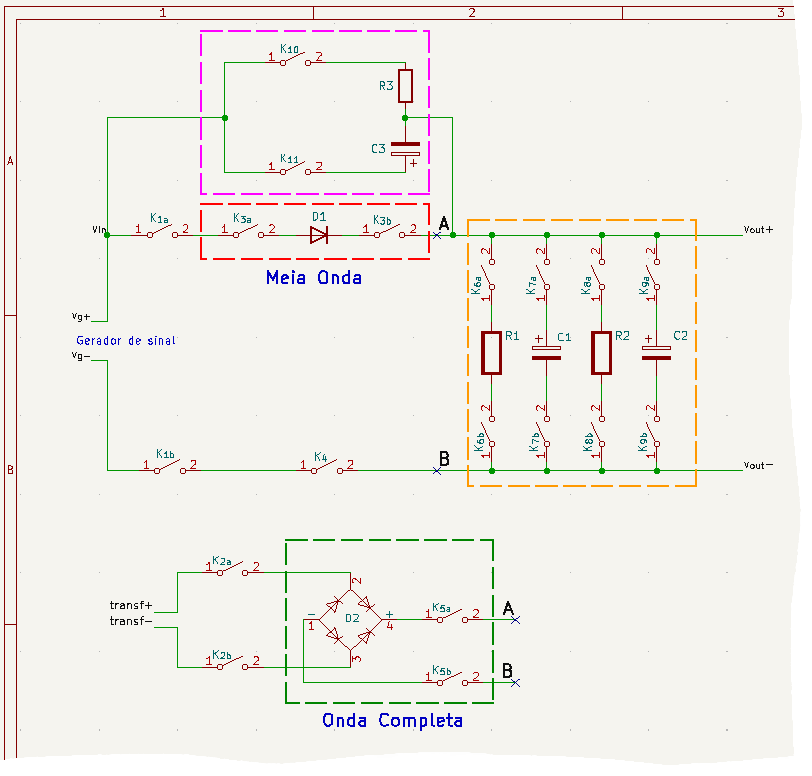
\includegraphics[width=0.5\textwidth]{figures/rec_fil_FULL.png}
	\caption{Esquema completo (simplificado) - rectificadores e filtros}
	\label{fig:rectificacao_filtragem_full}
\end{figure}

Na implementação dos rectificadores houve a necessidade de utilizar dois tipos de tensão de entrada. Como referido na Secção \ref{sec:fontesalimentacao}, o circuito de meia onda utiliza o gerador de sinal mas devido ao problema de massa, já explicado na mesma secção, foi necessário usar um transformador na rectificação de onda completa.

Na Figura \ref{fig:blocosrectificacao} está representado o diagrama de blocos geral da rectificação de meia e onda completa, (que pode ser aplicada)/aplicada, por exemplo, a uma fonte de tensão \acrshort{cc}.

\begin{figure}[hbtp]
	\centering
	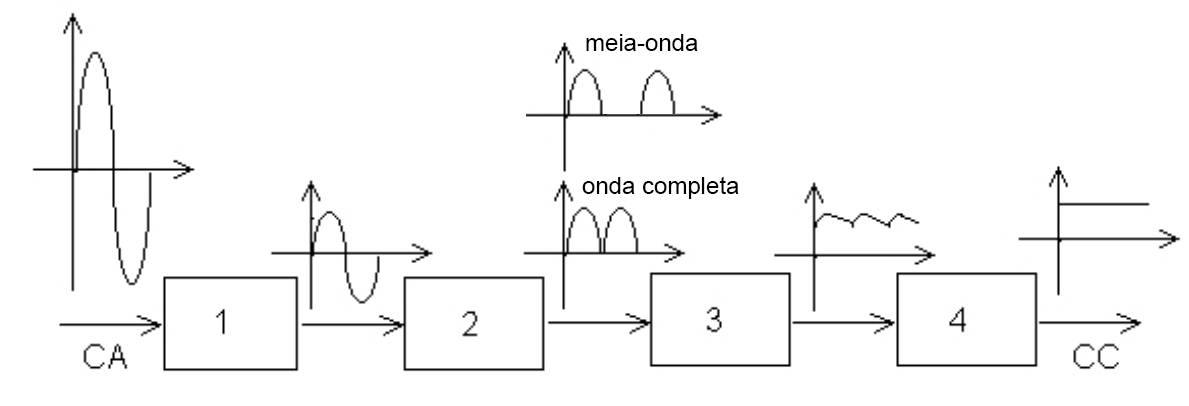
\includegraphics[width=0.7\textwidth]{figures/diagramablocosrectificacao.png}
	\caption{Diagrama de blocos geral da rectificação de meia e onda completa}
	\label{fig:blocosrectificacao}
\end{figure}

A Figura \ref{fig:placarectificadores} apresenta a implementação práctica das duas experiências na respectiva placa, pontos \ref{item2} a \ref{item7}. 

\begin{figure}[hbtp]
	\centering
	\includegraphics[width=0.5\textwidth]{figures/lare_rectificador_filtros_BLOCOS.png}
	\caption{Implementação práctica dos rectificadores e filtros}
	\label{fig:placarectificadores}
\end{figure}

%A implementação prática é composta pelos três blocos\footnote{A inclusão da estabilização poderá ser objecto de trabalho futuro.}, como se pode ver na Figura \ref{fig:placarectificadores}. 
\begin{enumerate}
	\item Bloco 1 - Implementado na placa da alimentação, representada no Figura \ref{fig:placartransformador} 
	\item \label{item2}Bloco 2 - Rectificação;
		\begin{enumerate}
			\item \label{diodos}Díodo rectificador ($1_{a}$) e Ponte rectificadora ($1_{b}$);	
		\end{enumerate}
	\item Bloco 3 - Filtragem \textins{componentes comuns a ambas as experiências};
		\begin{enumerate}
			\item \label{resistencias}Resistências (3);
			\item \label{condensadores}Condensadores (5);
		\end{enumerate}
	\item Relés (2);
	\item \textit{Drivers} de relés e registo de deslocamento (4);
	\item Ligação à placa seguinte através de conectores ``Arduino stackable'' (6);
	\item \label{item7}Resistência e condensador exclusivo dos filtros (7).
\end{enumerate}

\begin{figure}[hbtp]
	\centering
	\includegraphics[width=0.3\textwidth]{figures//lore_fonte.jpg}
	\caption{Transformador}
	\label{fig:placartransformador}
\end{figure}

Como referido na Secção \ref{sec:experiencias}, a implementação dos filtros foi realizada após a conclusão dos rectificadores. De forma a permitir a integração desta experiência no circuito já concluído, foi necessário realizar um \textit{bypass} ao díodo $D_{1}$ (assinalado pelo retângulo tracejado a vermelho na Figura \ref{fig:rectificacao_filtragem_full}). Esta alteração permitiu a introdução de uma resistência ($R_{3}$) ou de um condensador ($C_{3}$), consoante a configuração do filtro em estudo.

Os esquemas teóricos dos filtros estão representados nas Figuras \ref{fig:filtro_pb} e \ref{fig:filtro_pa}, sendo que $R$ e $C$  correspondem a $R_{3}$ e $C_{3}$.

Portanto, se se pretender estudar o filtro passa-baixo, é activado o relé $K_{10}$ ($R_{3}$) e o condensador de saída pode ser escolhido entre os $C_{1}$ e $C_{2}$, consoante a configuração que se pretende estudar. O mesmo se aplica ao filtro passa-alto, onde o relé $K_{11}$ ($C_{3}$) é activado e a resistência de saída pode ser escolhida entre os $R_{1}$ e $R_{2}$. 

Na Tabela \ref{Table:rectificadoresfiltros} e com o auxílio da Figura \ref{fig:rectificacao_filtragem_full} (ou do circuito completo apresentado no Anexo \ref{AppendixA}), pode ver-se o estado dos relés, respeitante a uma combinação possível para cada circuito. 

\begin{table}[htb]
	\centering
	\caption{Exemplo funcionamento do rectificador de meia onda} 
	\label{Table:rectificadoresfiltros}
	\resizebox{\columnwidth}{!}{\begin{tabular}{lccccccccccccc}
		\toprule
		               & \multicolumn{13}{c}{Estado dos relés} \\
		\midrule
		               			& $K_{1}$ & $K_{2}$ & $K_{3}$ & $K_{4}$ & $K_{5}$ & $K_{6}$ & $K_{7}$ & $K_{8}$ & $K_{9}$ & $K_{10}$ & $K_{11}$ & $K_{12}$ & $K_{13}$\\
		\midrule
		Meia Onda      			& 1		 	& 0       	& 1       & 1       & 0       & 1       & 1       & 0 	   & 0     		& 0       & 0       & 0 	   & 0 \\
		\midrule
		Onda Completa  			& 0 	 	& 1       	& 0       & 0       & 1       & 0       & 0       & 1  	   & 1    		& 0       & 0       & 1 	   & 1\\
		\midrule
		Filtro Passa-Alto      	& 1		 	& 0       	& 0       & 1       & 0       & 0       & 1       & 0 	   & 0    		& 1       & 0       & 1 	   & 1\\
		\midrule
		Filtro Passa-Baixo      & 1		 	& 0       	& 0       & 1       & 0       & 0       & 0       & 1 	   & 0    		& 0       & 1       & 1 	   & 1\\
		\bottomrule
	\end{tabular}}
\end{table}

\section{Software}
\label{sec:implementacaosoftware}
Hoje em dia vive-se (n)uma Era em que toda a informação está disponível na ``ponta dos dedos'' e à distância de um \textit{click}. A pesquisa, desenvolvimento e teste dos assuntos mais técnicos revelou-se longa e muitas vezes extenuante. Os recursos são (quase) incomensuráveis e o grande desafio foi tentar perceber a dicotomia certo/errado. Recorreu-se à Inteligência Artificial, documentação técnica \textit{online}, fóruns de discussão, ajuda pessoal, tutoriais \textit{online} e vídeos no YouTube.

Este projeto de código fonte aberto está dividido em dois repositórios, disponíveis para consulta e modificação sob a licença GPL-3.0 (GNU General Public License, versão 3) no GitHub: \href{https://github.com/eddygrinder/LaRE}{LaRE} e \href{https://github.com/eddygrinder/LaRE_PICode}{PiCode}. Assim, os ficheiros são referenciados relativamente ao respectivo repositório. Ao longo deste capítulo, sempre que se justificar e para fins de clareza, será apresentado o código necessário - em pequenos trechos - de forma a melhor ilustrar os conceitos discutidos. Não se pretende, contudo, abordar exaustivamente todas as instruções ou métodos de configuração do \acrshort{virtualbench}, sendo que os ficheiros se encontram devidamente comentados, sendo possível obter informações adicionais através da sua consulta. 

\subsection{Servidor Flask}
\label{sec:flask}
\textbf{Não sei se ainda vai ficar desta forma - no cap anterior já foi falada sobre a escolha do flask, por isso não faz sentido abordar novamente.}

Na Secção \ref{sec:back-end} foram já referidas as razões que levaram à escolha do \textit{Flask} como servidor \textit{web}. 

A base para a implementação do \textit{Flask} e \underline{\textbf{toda a informação descrita no}} \underline{\textbf{Capítulo \ref{sec:implementacaosoftware}}} teve como base e referência a documentação técnica disponível no \textit{site} do \href{https://flask.palletsprojects.com/en/3.0.x/}{\textit{Flask}} e complementada com alguns tutoriais do \textit{Youtube}, como por exemplo: \href{https://www.youtube.com/watch?v=dam0GPOAvVI}{\textit{link}} ou \href{https://www.youtube.com/watch?v=bB6Yyh7nUl4}{\textit{link}} .

\subsubsection{Estrutura base}
O fluxograma apresentado na Figura \ref{fig:funcflask} apresenta o funcionamento geral do servidor \textit{Flask}.

\begin{figure}[hbtp]
	\centering
	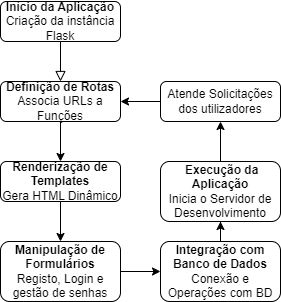
\includegraphics[width=0.7\textwidth]{figures/fluxograma_flask.drawio.png}
	\caption{Funcionamento geral \textit{Flask}}
	\label{fig:funcflask}
\end{figure}

A estrutura de directórios do \textit{Flask} tem uma base pré-definida que não é necessariamente rígida e pode ser adaptada consoante os requisitos do projecto \cite{Flask}. No caso do \acrshort{lare} a estrutura ficou organizada da forma como se mostra na Figura \ref{fig:estruturapastas}

\begin{figure}[hbtp]
	\centering
	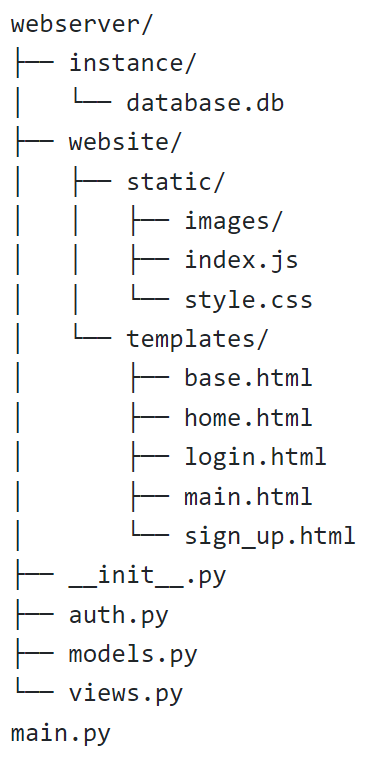
\includegraphics[width=0.3\textwidth]{figures/tree_flask.png}
	\caption{Estrutura de directórios - \textit{Flask} \textbf{ main.html está a mais}}
	\label{fig:estruturapastas}
\end{figure}

A raiz do projecto é o directório ``\textit{webserver}'' e nele estão contidos o ficheiro principal, assim como outros directórios e ficheiros de configuração essenciais:
\begin{itemize}
	\item \textit{main.py}: O ficheiro principal do aplicativo que inicializa e configura o \textit{Flask};
	\item \textit{requirements.txt}: Uma lista de dependências do projeto que podem ser instaladas usando \gls{pip};
	\item \textit{static/}: Este directório contém os ficheiros estáticos como \acrshort{css}, \textit{JavaScript} e as imagens usadas em toda a aplicação;
	\item \textit{templates/}: Contém os modelos \acrshort{html} usado para renderizar as visualizações;
	\item \textit{instance/}: Diretório para armazenar ficheiros de configuração ou ficheiros que mudam em tempo de execução, específicos da cada instância, por exemplo, ficheiros da base de dados.
\end{itemize}

Dentro da raiz, criou-se o directório \textit{website} onde se incluiu os ficheiros respeitantes ao funcionamento do \textit{site}. Nele constam os já descritos \textit{templates}, \textit{static} e ainda os seguintes ficheiros:

\begin{itemize}
	\item \textit{\_\_init\_\_.py}: Inicializa o \textit{Flask} e define as configurações. Este ficheiro dentro da directoria \textit{website} faz com que esta seja tratada como um pacote \textit{Python}. Isto quer dizer que a directoria pode ser importada e tudo o que estiver dentro é executado automaticamente;
	\item \textit{views.py}: Contém as funções de visualização para o tratamento de pedidos \acrfull{http};
	\item \textit{models.py}: Define os modelos de dados para a aplicação;
	\item \textit{auth.py}: Este ficheiro é responsável por lidar com a autenticação e autorização de utilizadores, pode incluir funções e rotas que permitem aos utilizadores registarem-se, fazer \textit{login} e fazer \textit{logout}.
\end{itemize}

\subsubsection{Rotas}
As aplicações \textit{Web} modernas utilizam \acrshort{url}s amigáveis para ajudar os utilizadores a memorizar e utilizar o nome para voltar a visitar diretamente uma página.

No \textit{Flask} utiliza-se o decorador \textit{\textbf{route()}} para associar uma função a um \acrshort{url}, tal como pode ser visto na Listagem \ref{lst:decoradorroute}.

\begin{minipage}{0.9\linewidth}
	\begin{lstlisting}[language=Python, caption=Decorador \textit{route()} - \textit{views.py}, label=lst:decoradorroute]
@views.route("/ohm", methods=['GET', 'POST'])
@login_required
def pagina_seguinte():
    return render_template("ohm.html", user=current_user)
\end{lstlisting}
\end{minipage}

O decorador \textit{\textbf{route}} define uma rota para a \acrshort{url} \textit{ohm}. Esta rota aceita pedidos \acrshort{http} de métodos \textit{GET} e \textit{POST}.

O decorador \textit{\textbf{login}} garante que o utilizador tem de estar autenticado para aceder a esta rota. Se o utilizador não estiver autenticado, será redirecionado para a página de \textit{login}.

A função pagina\_seguinte() é executada assim que a respectiva rota for acedida.

A última linha renderiza o \textit{template} \textit{\textbf{home.html}} e passa o objecto \textit{current\_user} para o \textit{template}.

Para construir um \acrshort{url} para uma função específica, usa-se a função \textit{\textbf{url\_for()}}. Esta função aceita o nome da função como seu primeiro argumento e qualquer número de argumentos de palavras-chave, cada um correspondendo a uma parte variável da regra de \acrshort{url}, tal como pode ser visto na Listagem \ref{lst:urlfor}

\begin{minipage}{0.9\linewidth}
	\begin{lstlisting}[language=Python, caption=Contrução de \textit{url}s - \textit{auth.py}, label=lst:urlfor]
(...)
if user:
    if check_password_hash(user.password, password):
        flash('Logged in successfully!', category='success')
        login_user(user, remember=True)
        return redirect(url_for('views.home'))
(...)
\end{lstlisting}
\end{minipage}

Isto quer dizer que o \textit{Flask} gera a \acrshort{url} correspondente à função \textit{\textbf{home()}} definida no ficheiro \textit{\textbf{views.py}} dentro da \textit{Blueprint} \textit{views}. Quando usada dentro de \textit{\textbf{redirect}}, redireciona o utilizador para essa \acrshort{url}.

\subsubsection{Blueprints}
O \textit{Flask} usa um conceito de \textit{blueprints} para criar componentes de aplicações e suportar padrões comuns dentro de uma aplicação ou entre aplicações. As \textit{blueprints} podem simplificar muito o funcionamento de grandes aplicações e fornecer um meio central para que as extensões do \textit{Flask} registem operações em aplicações. As \textit{blueprints} permitem organizar a aplicação em partes menores e de mais fácil gestão. O conceito básico das \textit{blueprints} é que registam as operações a executar quando são integrados numa aplicação. O \textit{Flask} associa funções de vista (\textit{views}) a \textit{blueprints} quando processa pedidos e gera \acrshort{url} entre diferentes pontos de acesso.

Na Listagem~\ref{lst:blueprintviews} e Listagem~\ref{lst:blueprintauth} podem ver-se as duas \textit{blueprints} definidas no caso da implementação do \acrshort{lare}.
\begin{center}
	\begin{minipage}{0.7\linewidth}
		\begin{lstlisting}[language=Python, caption=\textit{Blueprint views} - \textit{views.py}, label=lst:blueprintviews]
views = Blueprint('views', __name__)
\end{lstlisting}
	\end{minipage}
\end{center}

\begin{center}
	\begin{minipage}{0.7\linewidth}
		\begin{lstlisting}[language=Python, caption=\textit{Blueprint auth} - \textit{auth.py}, label=lst:blueprintauth]
auth = Blueprint('auth', __name__)
\end{lstlisting}
	\end{minipage}
\end{center}

Ambas as \textit{blueprints} são registadas no ficheiro \textit{\_\_init\_\_.py}, como se pode verificar na Listagem \ref{lst:initreg}

\begin{center}
	\begin{minipage}{0.7\linewidth}
		\begin{lstlisting}[language=Python, caption=Registo das \textit{blueprints} - \textit{\_\_init\_\_.py}, label=lst:initreg]
app.register_blueprint(views, url_prefix='/')
app.register_blueprint(auth, url_prefix='/')
\end{lstlisting}
	\end{minipage}
\end{center}

Isto quer dizer que ao registar a \textit{blueprint} com o prefixo ``/'', os \acrshort{url}s serão acessíveis através da raiz da aplicação.

\subsubsection{Pedidos}
A capacidade de uma aplicação \textit{web} em responder a solicitações de dados do cliente é um requisito essencial. No \textit{Flask} esta informação é fornecida pelo objeto global \textit{\textbf{request}}. Este objeto contém todos os detalhes da solicitação, como os métodos \acrshort{http} usados (\textit{GET}, \textit{POST}, etc.), os \textit{headers} os \textit{cookies} ou o corpo da requisição.

O método de requisição pode ser determinado através do atributo \textit{\textbf{method}}. Para aceder aos dados de um formulário (transmitidos numa requisição \textit{POST} ou \textit{PUT}), utiliza-se o atributo \textit{\textbf{form}}, tal como descrito no ficheiro auth.py.

Quando se adiciona um ponto de interrogação (?) seguido de pares chave-valor (key=value) no final de um \acrshort{url}, está a enviar-se dados adicionais ao servidor, esses dados são chamados de \textbf{parâmetros do \acrshort{url}}, como se pode ver na Listagem \ref{lst:paramurl}.

\begin{minipage}{0.9\linewidth}
	\begin{lstlisting}[language=Html, caption=Exemplo argumentos passados ao servidor - ohm.html, label=lst:paramurl]
const url = `/config_VirtualBench?parameter=${parameter}&Vcc=${Vcc}&R=${Resistance}`;
\end{lstlisting}
\end{minipage}

No entanto, a criação e renderização das páginas \acrshort{html} é feita automaticamente através dos modelos \textit{Jinja2}\footnote{A documentação pode ser consultada em \href{https://jinja.palletsprojects.com/en/3.1.x/templates/}{\textit{Jinja}}}. Os modelos podem ser usados para gerar qualquer tipo de ficheiro de texto, sendo que para aplicações \textit{web} serão, principalmente, páginas \acrshort{html}.

No ficheiro base.html, pode ver-se a combinação entre código \acrshort{html} e sintaxe \textit{Jinja2}.

No código \acrshort{html}, encontram-se secções entre chavetas {} com palavras-chave especiais como por exemplo {\% block \%} e {\% endblock \%}. Estes são blocos de modelo \textit{Jinja2} que definem áreas de conteúdo dinâmico que podem ser preenchidas com lógica ou dados em \textit{Python}. Para renderizar um modelo, o método utilizado foi \textit{\textbf{render\_template()}} \cite{Flask}. O \textit{Flask} procurará por modelos na pasta \textit{templates}, como pode ser visto na Figura \ref{fig:estruturapastas}.

Na página oficial do \textit{Flask} é recomendado que se aceda aos parâmetros do \acrshort{url} com \textit{\textbf{get}} ou capturando o \textit{\textbf{KeyError}}, uma vez que os utilizadores podem alterar o \acrshort{url} e, nesse caso, apresentar uma página \textit{400 bad request} não é de fácil interpretação. \textbf{ATENÇÃO: Verificar se será preciso desenvolver mais este parágrafo - OPINIÃO PROF}

\subsubsection{Base de dados}
A aplicação desenvolvida usa uma base de dados e autenticação de utilizador, a ligação com a base de dados é aberta no início do pedido e é obtida a informação do utilizador. No final do pedido, a ligação com a base de dados é fechada.

No contexto da documentação do \textit{Flask} e implementação de uma base de dados, são apresentados duas alternativas: \textit{SQLite 3} e \textit{SQLAlchemy}. Tal como referenciado/aconselhado na documentação, usou-se a extensão \textit{Flask-SQLAlchemy}, descrita no ficheiro \textit{\textunderscore\textunderscore init.py\textunderscore\textunderscore}.

\subsubsection{Autenticação}
A segurança da aplicação é assegurada através das funcionalidades de \textit{login} e \textit{logout}, implementadas no ficheiro \textit{auth.py}. Para tal, foi instalada a extensão \textit{flask-login}.

Esta extensão facilita a gestão de sessões de utilizadores, permitindo manter o estado autenticado entre diferentes requisições, fornecendo métodos como \textbf{\textit{login\textunderscore user()}}, \textbf{\textit{logout\textunderscore user()}} e \textbf{\textit{current\textunderscore user}}, que simplificam a verificação do estado de autenticação. O processo de registo envolve a recolha de credenciais, como nome de utilizador e senha, garantindo o armazenamento seguro da senha através de \textbf{\textit{hashing}} com \textbf{\textit{generate\textunderscore password\textunderscore hash}}. No \textit{login}, a aplicação verifica as credenciais fornecidas, compara a senha inserida com a armazenada usando \textbf{\textit{check\textunderscore password\textunderscore hash}} e, se for válida, inicia a sessão do utilizador. Além disso, certas rotas são protegidas para garantir que apenas utilizadores autenticados as possam aceder, utilizando o decorador \textbf{\textit{@login\textunderscore required}}, que redireciona utilizadores não autenticados para a página de \textit{login}. A gestão de sessões é feita através de \textit{cookies} seguros, permitindo ainda a funcionalidade de lembrar a sessão entre reinícios do navegador, caso seja activado o parâmetro \textbf{\textit{remember=True}} no \textbf{\textit{login\textunderscore user}}. 

Devido à complexidade da implementação de uma verificação por \textit{email}, a aplicação restringe-se à autenticação baseada apenas no nome de utilizador e senha. A inclusão desse mecanismo exigiria um serviço de envio de \textit{emails} e a gestão de \textit{tokens} de confirmação.

\textbf{A REVER: Valerá a pena uma página de admin, de forma a que o professor, por exemplo faça os registo e forneça os dados de acesso aos alunos?}

\subsection{Arquitectura de Comunicação}
\label{sec:comunicacao}
Nesta secção, o foco será analisar a comunicação (e troca de parâmetros) entre os diversos tipos de ficheiros. Na Figura \ref{fig:diagramasimplificado} é apresentado o diagrama simplificado que ilustra o funcionamento geral deste tipo de comunicação. 

\begin{figure}[hbtp]
	\centering
	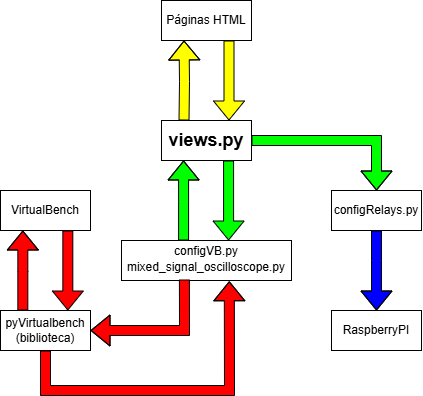
\includegraphics[width=0.7\textwidth]{figures/Diagrama_simplificado.drawio.png}
	\caption{Diagrama de comunicação simplificado [REVER]}
	\label{fig:diagramasimplificado}
\end{figure}

A arquitectura do sistema é composta por multiplos ficheiros que comunicam entre si, englobando a troca de parâmetros. O critério utilizado foi o de manter o ficheiro \textit{views.py} o mais leve e simples possível, mantendo-se o comando e controlo dos dispostivos em ficheiros separados.

Como mencionado na Secção \ref{sec:flask}, a estrutura de directórios do \textit{Flask} possui uma base pré-definida, mas suficientemente flexível para ser adaptada conforme os requisitos específicos do projeto, como ilustrado na Figura \ref{fig:estruturapastas}. De uma forma geral, foram criados ficheiros específicos para cada experiência, adoptando o critério de evitar uma excessiva modularização do código. Embora esta prática ofereça vantagens, também apresenta as suas desvantagens - devido à fragmentação excessiva - já que pode tornar a compreensão e manutenção do código mais complexa.

Os seguintes ficheiros foram criados e associados às respectivas experiências:

\textbf{Específicos}
\begin{itemize}
	\item Lei de \textit{Ohm} - \textit{config.py};
	\item Rectificadores/Filtros - \textit{mixed\_signal\_oscilloscope.py};
	\item \textins{ohm, meiaonda, ondacompleta, passaalto, passabaixo}.html.
\end{itemize}

\textbf{Comuns}
\begin{itemize}
	\item \textit{views.py} - parte central da aplicação, pois nele estão definidas todas as rotas \textit{Flask}. Quer isto dizer que, cada roda representa uma funcionalidade ou página \textit{web} específica e qualquer troca de dados ou argumentos entre ficheiros e/ou \textit{scripts}, passa obrigatoriamente por este ficheiro. Sendo assim, tentou-se, sempre que possível, reduzir o código ao estritamente necessário;
	\item \textit{configRelays.py} - ficheiro responsável pelo envio da trama de \textbf{bits} para o \textit{RaspberryPI}.
	\item \textins{login, base, sign\_up}.html - páginas de autenticação e registo de utilizadores.
\end{itemize}

\subsubsection{Comunicação entre ficheiros}
\label{sec:comunicacaoentrefich}
A comunicação entre as páginas \acrshort{html} e o ficheiro \textit{python}\footnote{Pode-se, neste caso, reduzir a comunicação ao caso mais geral de troca de informação entre ficheiros \acrshort{html} e \textit{python}, já que, no fundo, o ficheiro \textit{views.py} está escrito em \textit{python}.} é feita nos dois sentidos - setas amarelas - já que os utilizadores enviam os parâmetros específicos de cada experiência e os resultados são apresentados nas páginas. 

A Listagem \ref{lst:htmlpy} ilustra a forma como os parâmetros são enviados da página \acrshort{html} para o ficheiro \textit{python}, através de uma \textit{query string}.

\textbf{Aqui poderia ficar o parágrafo da explicação do ?}

\begin{minipage}{0.9\linewidth}
	\begin{lstlisting}[language=html, escapechar=|, caption=Envio de parâmetros \acrshort{html} $\rightarrow$ \textit{views.py}, label=lst:htmlpy]
	const url = `/config_VirtualBench?variavel_1=${parametro_1}&variavel_2=${parametro_2}&variavel_3=${parametro_3}`; |\label{line:parametros}|
	\end{lstlisting}
\end{minipage}

Do lado do servidor, o \textit{Flask} disponibiliza o objecto \textit{request}, a partir do qual os parâmetros enviados por \acrshort{url} podem ser acedidos através da função \textit{request.args.get()}, como representado na Listagem~\ref{lst:metodorequest}.

\begin{minipage}{0.9\linewidth}
	\begin{lstlisting}[language=python, escapechar=|, caption=Recepção de parâmetros, label=lst:metodorequest]
		Vcc = request.args.get('parametro_1', 0, int)  |\label{line:vccrequest}|
	\end{lstlisting}
\end{minipage}

O envio de parâmetros do ficheiro \textit{python} para as páginas \acrshort{html} é feito em \acrfull{json}, usando a instrução definida na Listagem \ref{lst:returnjson}.

\begin{minipage}{0.9\linewidth}
	\begin{lstlisting}[language=python, escapechar=|, caption=Envio de parâmetros \textit{views.py} $\rightarrow$ \acrshort{html}, label=lst:returnjson]
		return jsonify({'measurement_result': measurement_result})
	\end{lstlisting}
\end{minipage}

Do lado das páginas \acrshort{html} a recepção do resultado é feita através do método \textit{fetch()}, como se pode ver na Listagem \ref{lst:recepcaojson}.

\begin{minipage}{0.9\linewidth}
	\begin{lstlisting}[language=html, escapechar=|, caption=Recepção de parâmetros, label=lst:recepcaojson]
		fetch(url)
		.then((response) => response.json())
		// Aceder a variavel measurement_result
		.then((data) => {
		  document.getElementById("current-measure").innerHTML = 
		  	data.measurement_result + " mA";	
		\end{lstlisting}
\end{minipage}

As setas verdes representam a comunicação entre dois ficheiros \textit{python}. O processo é bastante simples, bastando para isso, importar o ficheiro que contém a função que se pretende chamar. A Lista \ref{lst:pypy} ilustra a forma como se importa um ficheiro \textit{python} e a chamada da respectiva função com o parâmetro a passar.

\begin{minipage}{0.9\linewidth}
	\begin{lstlisting}[language=python, escapechar=|, caption=Comunicação \textit{python} - \textit{python}, label=lst:pypy]
		from ctrl_hardware import configRelays, configVB, mixed_signal_oscilloscope |\label{line:ficheiros}|
		configRelays.config_relays_ohm(Resistance, measure_parameter) |\label{line:trueparameter}|
	\end{lstlisting}
\end{minipage}

No entanto, o caso das medições no âmbito da Lei de \textit{Ohm} reveste-se de particularidades. A Figura~\ref{fig:processoleituraUI} ilustra o processo de leitura das medições de tensão e corrente.

\begin{figure}[hbtp]
	\centering
	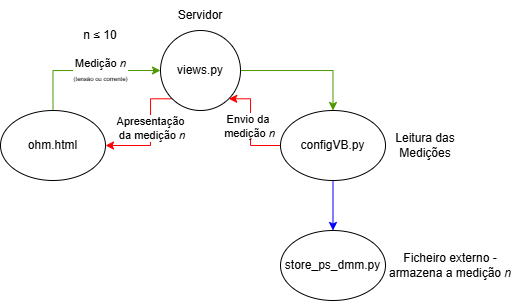
\includegraphics[width=0.7\textwidth]{figures/medicoes_OHM.drawio.png}
	\caption{Processo de leitura das medições de tensão e corrente}
	\label{fig:processoleituraUI}
\end{figure}

As setas a verde e vermelho representam o fluxo do processo iniciado pelo utilizador ao solicitar uma medição. Este ciclo repete-se cinco vezes para cada grandeza (tensão e corrente). No entanto, como o ficheiro \textit{configVB.py} é executado de forma independente em cada chamada, num total de dez execuções, os valores medidos não são retidos entre invocações sucessivas.

Para contornar esta limitação e garantir a persistência das medições ao longo das múltiplas chamadas à \acrshort{api}, sem recorrer a mecanismos clássicos de persistência, como ficheiros \textit{.json}, \textit{.csv} ou bases de dados locais, que implicariam operações de escrita/leitura ao sistema de ficheiros, foi desenvolvido um módulo auxiliar em Python, implementado no ficheiro \textit{store\_ps\_dmm.py}. Este módulo utiliza variáveis globais como mecanismo de armazenamento em memória. Os valores de tensão e corrente são armazenados num \textit{array} através da função \textit{np.append}, da biblioteca \textit{NumPy} \cite{NumPy}.

Dado que o servidor \textit{Flask} se mantém activo durante todo o processo de medição, as variáveis globais permanecem acessíveis em memória entre chamadas à \acrshort{api}. Esta abordagem simplifica a gestão do estado da aplicação numa fase inicial de desenvolvimento, sendo eficaz enquanto o processo da aplicação não for reiniciado.


\subsubsection{Comunicação com RaspberryPi}
\label{sec:raspberrypi}
Do lado do \textit{Raspberry Pi}, embora de uma forma mais simples, também se usou a premissa de modularização do código, tal como referido na Secção \ref{sec:comunicacao}. Este ficou dividido em dois ficheiros:
\begin{itemize}
	\item \textit{receive.py} - recebe a \textit{string};
	\item \textit{shift\textunderscore register.py} - responsável por activar os relés.
\end{itemize}

A comunicação com o \textit{Raspberry Pi} é estabelecida através de sockets, um método já descrito na Secção~\ref{sec:arquitectura}. Após a configuração e teste dos parâmetros, uma \textit{string} representando o número de relés a ativar - 8 \textit{bits} ou 13 \textit{bits}, dependendo dos circuitos - é enviada através da \textit{interface} de rede. A implementação do mecanismo de comunicação encontra-se no ficheiro \textit{configRelays.py}, na função \textit{config\textunderscore Relays}.

Sendo assim, o ficheiro \textit{receive.py} é executado inicialmente e aguarda pela envio da \textit{string}. De referir que, embora o \textit{socket} esteja configurado em \textit{blocking mode} - quer isto dizer que o cliente ficará bloqueado na Linha~\ref{line:blockmode}, da Listagem \ref{lst:socketblock}, esperando uma resposta do servidor \cite{Sockets} (acontece enquanto a string não for enviada) - optou-se por enviar uma confirmação do servidor ao cliente. Não sendo estritamente necessário, foi adicionada como auxílio à depuração.

\begin{minipage}{0.9\linewidth}
	\begin{lstlisting}[language=Python,escapechar=|, caption=\textit{Block Mode \textins{Sockets} configRelays.py}, label=lst:socketblock]
		# Espera pela resposta do servidor
        while True:
            data = s.recv(1024) |\label{line:blockmode}|
            if not data:
                break
            response = data.decode()
            if response == 'True':  # Espera por uma confirmacao especifica do servidor
                print("Confirmacao recebida do servidor:", response)
                break
	\end{lstlisting}
\end{minipage}

O passo final é a activação dos relés, realizada no ficheiro \textit{shift\textunderscore register.py}, função \textit{commandRelays}. O procedimento foi descrito na Secção \ref{sec:hwregistodeslocamento}, sendo que os modos de funcionamento estão representados na Tabela \ref{Table:funcSN74HC595}.

Para que as experiências funcionem correctamente, todos os relés terão de ser activados ao mesmo tempo. Isto requer que à \textit{string} seja feito um \textit{and bit} a \textit{bit} - \textbf{NOTA: Se calhar explicar melhor como é formada a string, no fundo não é uma string mas uma trama de bits} e cada um deles enviado para o registo de deslocamento, numa configuração \acrshort{sipo}, tal como pode ser visto na Listagem \ref{lst:andbitabit}. Assim que os 8 \textit{bits} ou 13 \textit{bits} forem todos tranferidos para o registo, será activada a saída paralela e o relés activados. \textbf{A REVER: trocar o termo string por trama?} 

\begin{minipage}{0.9\linewidth}
	\begin{lstlisting}[language=Python,escapechar=|, caption=\textit{And bit} \textit{bit shift\textunderscore register - NOME DO FICH}, label=lst:andbitabit]
		for i in range(n_bits):
			binaryShift = binaryString & 1
			if binaryShift == 1:
				WriteReg (ON, SERCLK_pin_ctrl, SER_pin_ctrl, WaitTimeSR)
			else:
				WriteReg(OFF, SERCLK_pin_ctrl, SER_pin_ctrl, WaitTimeSR)
			binaryString = binaryString >> 1
		OutputReg(RCLK_pin_ctrl)
		return True # Fim da transmissao da trama de bits, reles activados
	\end{lstlisting}
\end{minipage}

\subsubsection{VirtualBench - Configurações e medições}
\label{sec:configmedicaoes}
O comando e controlo do \acrshort{virtualbench} (e respectivos instrumentos) é realizado através da biblioteca \textit{pyVirtualBench}\footnote{No \textit{site} - \href{https://pymeasure.readthedocs.io/en/latest/api/instruments/ni/virtualbench.html}{\textit{link}} - está incluída documentação detalhada sobre a biblioteca \textit{pyVirtualBench} e os métodos disponíveis para cada instrumento.\label{fnlabel}} - representado na Figura~\ref{fig:diagramasimplificado} pelas setas vermelhas - que, como já foi referido na Secção \ref{sec:solucaoproposta}, é um \textit{wrapper} que permite controlar o \acrshort{virtualbench} a partir de uma aplicação \textit{Python}.

Além de instalar a biblioteca, os autores disponibilizam uma série de exemplos, sendo que, aqueles que mais se adequam aos objectivos deste projecto são:
\begin{itemize}
	\item \textit{dmm\_example.py}: exemplo que demonstra como efetuar medições utilizando o multímetro digital;
	\item \textit{fgen\_example.py}: exemplo que demonstra como configurar e gerar uma onda através do gerador de sinal;
	\item \textit{mso\_simple\_example.py}: exemplo que demonstra como configurar e adquirir dados do osciloscópio, utilizando a funcionalidade de configuração automática incorporada;
	\item \textit{ps\_example.py}: exemplo que demonstra como efetuar medições utilizando a fonte de alimentação.
\end{itemize}

De forma a realizar as configurações e medições do \acrshort{virtualbench}, tomou-se como ponto de partida os exemplos já fornecidos com a biblioteca \textit{pyVirtualBench} e adaptaram-se ao contexto do projecto. 

Nesta secção, apresenta-se como exemplo a configuração da fonte de alimentação, por ser o único instrumento utilizado em todas as experiências realizadas. 

Como referido na Secção \ref{sec:comunicacaoentrefich}, nota de rodapé \footref{fnlabel}, a documentação da biblioteca, bastante completa e detalhada, está disponível para consulta no referido \textit{link}, pelo que se aconselha a sua consulta para mais informações \textbf{??}. 

Através da análise dos exemplos disponibilizados para o \acrshort{virtualbench} (e que estão definidos no repositório já mencionado do \textit{GitHub}), foi possível compreender a estrutura geral de configuração aplicada aos instrumentos e fontes de alimentação. Com base nessa análise, determinou-se a seguinte lógica de funcionamento:

\begin{enumerate}
	\label{item:logica}
	\item Aquisição do \textit{virtualbench};
	\item Aquisição dos instrumentos;
	\item Configurações específicas de cada instrumento;
	\item Desenvolvimento do programa;
	\item Libertar os instrumentos;
	\item Libertar o \textit{virtualbench}.
\end{enumerate}

A aquisição do \acrshort{virtualbench}, identificado como \textit{VB8012-30A210F}, é feita através da criação de uma instância da classe \textit{PyVirtualBench}, que é a classe principal da biblioteca \textit{pyVirtualBench}, definida na Linha \ref{line:vb8012}, da Listagem \ref{lst:instanciacao}.

\begin{center}
\begin{minipage}{0.9\linewidth}
	\begin{lstlisting}[language=Python,escapechar=|, caption=Instanciação da classe \textit{PyVirtualBench}, label=lst:instanciacao]
		virtualbench = PyVirtualBench('VB8012-30A210F') |\label{line:vb8012}|
		ps = virtualbench.acquire_power_supply() |\label{line:acquireps}|
	\end{lstlisting}
\end{minipage}
\end{center}

A partir do objeto \textit{virtualbench}, é possível aceder aos diferentes instrumentos, sendo que a aquisição é feita através do método \textit{acquire\_\textless instrumento\textgreater()}. Essa instância é armazenada numa variável definida pelo utilizador, permitindo o acesso às funcionalidades de configuração, controlo e medição disponibilizadas por esse instrumento. Na Listagem \ref{lst:instanciacao}, linha \ref{line:acquireps}, pode ver-se, a título de exemplo, como é feita a aquisição da fonte de alimentação, que é armazenada na variável \textit{ps}.

Um exemplo da configuração da fonte está descrita na Listagem \ref{lst:exemploconfigps}

\begin{minipage}{0.7\linewidth}
	\begin{lstlisting}[language=Python,escapechar=|, caption=Exemplo \textit{ps\_example.py}, label=lst:exemploconfigps]
		try:
			# Configuracao da fonte de alimentacao
			channel = "ps/+25V" |\label{line:channel}| 
			voltage_level = 1.0 |\label{line:voltagelevel}|
			current_limit = 0.5 |\label{line:currentlimit}|
			# Configuracao especifica
			ps.configure_voltage_output(channel, voltage_level, current_limit)|\label{line:configvoltage}|
			ps.enable_all_outputs(True)|\label{line:enableoutputs}|
	\end{lstlisting}
\end{minipage}

\begin{itemize}
	\item \textit{channel} - linha \ref{line:channel}: especifica o canal da fonte de tensão a utilizar, sendo que, neste exemplo, é selecionado o canal de \SI{25}{\volt}, através do nome ``ps/+25V'' (podendo também ser utilizado ``ps/+6V'' para o canal de \SI{6}{\volt});
	\item \textit{voltage\_level} - linha \ref{line:voltagelevel}: define o valor da tensão de saída. No caso deste exemplo, \SI{1.0}{\volt}. Pode ser, também, atribuída uma variável - $V_{cc}$ - com base nos valores apresentados na Figura~\ref{fig:pagohm});
	\item  \textit{current\_limit} - linha \ref{line:currentlimit}: é configurado o limite de corrente para \SI{0.5}{\ampere};
	\item \textit{ps.configure\_voltage\_output(channel, voltage\_level, current\_limit)} - linha \ref{line:configvoltage}: configura a fonte de alimentação com os parâmetros definidos nas linhas \ref{line:channel} a \ref{line:currentlimit};
	\item \textit{ps.enable\_all\_outputs(True)} - linha \ref{line:enableoutputs}: ativa todas as saídas da fonte de alimentação. No entanto, só a saída correspondente ao canal definido na linha \ref{line:channel} será ativada.
\end{itemize}

No final da execução, os instrumentos e o \acrshort{virtualbench} têm de ser libertados, por esta ordem. Isto é feito através do método \textit{instrumento.release()}. Se tal não for feito, o \acrshort{virtualbench} e os instrumentos chamados não serão libertados, ficando inacessíveis para futuras chamadas. \textbf{A REVER: dar um exemplo do que acontece??}

De referir que vários instrumentos podem ser chamados simultaneamente e, para cada um deles, assim como para o \acrshort{virtualbench}, é criada uma instância para o respectivo objecto, cuja referência corresponde a um endereço de memória. 

O resultado das instruções na Linha~\ref{line:acquireps} e Linha~\ref{line:vb8012} da Listagem~\ref{lst:instanciacao} é:
\begin{itemize}
	\item (...)PyVirtualBench object at 0x000001E7DEECAD20.
	\item (...)PyVirtualBench.PowerSupply object at 0x000001E7DEECB2F0;
\end{itemize}

No entanto, se um ficheiro for chamado várias vezes (como no caso da experiência da Lei de \textit{Ohm}), uma nova instância do instrumento será sempre criada a cada chamada. Além disso, se houver várias funções no mesmo ficheiro, os objetos criados (por exemplo, 0x000001E7DEECAD20) devem ser passados entre funções ou, alternativamente, o instrumento deve ser encerrado e reinicializado entre chamadas de funções. \textbf{voltar a verificar isto}

\subsubsection{Gráficos}
\label{sec:graficos}
Os gráficos apresentados são gerados com recurso às bibliotecas \textit{NumPy} \cite{NumPy} e \textit{Matplotlib} \cite{Matplotlib}, amplamente utilizadas em \textit{Python}. 

A \textit{NumPy} é uma biblioteca fundamental para computação científica, permitindo a manipulação eficiente de \textit{arrays} multidimensionais e fornecendo um vasto conjunto de funções matemáticas, estatísticas e de álgebra linear. No contexto da construção de gráficos, o \textit{NumPy} é essencial na preparação e transformação dos dados a representar. O declive da recta obtido experimentalmente, no estudo da Lei de \textit{Ohm}, representado na Listagem \ref{lst:decliverecta}, foi calculado com recurso à biblioteca \textit{SciPy}, que disponibiliza ferramentas avançadas de análise científica, incluindo ajustamento de curvas e complementa a \textit{NumPy}, sobre a qual está construída.

\begin{minipage}{0.9\linewidth}
	\begin{lstlisting}[language=Python,escapechar=|, caption=Cálculo do declive da recta, label=lst:decliverecta]
		slope, intercept, r_value, p_value, std_err = stats.linregress(voltage_measurements, current_measurements)
	\end{lstlisting}
\end{minipage}

A visualização dos dados é realizada através da \textit{Matplotlib}, uma biblioteca consolidada para criação de gráficos em \textit{Python}. Esta permite gerar representações visuais, como gráficos de linhas, dispersão, histogramas, entre outros. Neste projecto, a \textit{Matplotlib} é utilizada para representar de forma clara e interpretável os dados e resultados obtidos. A Listagem \ref{lst:graficoUvsI} ilustra a forma como se gera um gráfico experimental correspondente à Lei de \textit{Ohm}.

\begin{minipage}{0.9\linewidth}
	\begin{lstlisting}[language=Python,escapechar=|, caption=Gráfico Corrente \textit{vs} Tensão, label=lst:graficoUvsI]
		plt.plot(voltage_measurements, current_measurements, label='V Vs I', marker = 'o')
	\end{lstlisting}
\end{minipage}

Outro tipo de gráficos que são gerados são os diagramas de Bode, que representam a resposta em frequência dos filtros. A Listagem \ref{lst:diagramaBode} ilustra a forma como são gerados os pontos das frequências para o gráfico de Bode. Neste caso, as frequências são geradas logaritmicamente, utilizando a função \textit{logspace} da biblioteca \textit{NumPy}.

\begin{minipage}{0.9\linewidth}
	\begin{lstlisting}[language=Python,escapechar=|, caption=Filtros - Diagrama de \textit{Bode}, label=lst:diagramaBode]
		num_points = int(np.log10(stop_freq / start_freq) * points_per_decade)
		frequencies = np.logspace(np.log10(start_freq), np.log10(stop_freq), num=num_points)	
	\end{lstlisting}
\end{minipage}

As imagens geradas são gravadas na pasta ``webserver/website/static/images/'', tal como indica o exemplo na Listagem \ref{lst:gravacaoimagem}. 

\begin{minipage}{0.9\linewidth}
	\begin{lstlisting}[language=Python,escapechar=|, caption=Gravação do gráfico, label=lst:gravacaoimagem]
	    plt.savefig("webserver/website/static/images/ohm_graph.png")	
	\end{lstlisting}
\end{minipage}

\subsection{Interface WEB}
\label{sec:interfaceweb}
\textbf{NOTA: Acho que esta secção precisa de ser revista?? melhorada??}

%Resumindo Na experiencia da lei de ohm há o controlo dos valores da experiêncianeuica, medições a apresentação do gráfico. Este gráfico só é apresentado quando o utilizador carregar no respectivo link. Nas outras experiências, como o utilizador já tem menos controlo - só controla a frequência - REFERIR COMO É APRESENTADO O GRÁFICO. NÃO ESQUECER DO DIAGRAMA DE BODE.

%FALAR DA PARTE HTML PARA DEPOIS EMBARCAR NA TROCA DE DADOS,  FALTA A PARTE DA COMUNICAÇÃO COM O pi.

%ORGANIZAÇÃO DOS FICHEIROS, A FUNCÇÃO DE CADA FICHEIRO OU SCRIPT, NÃO ESQUECER O PI5, COMO É FEITA A COMUNICAÇÃO ENTRE OS SCRIPS, É DIFERENTE NAS VÁRIAS EXPERIÊNCIAS.

%Há um ficheiro central que ``controla'' todas as rotas \textit{flask} - views.py.
%Talvvez colocar um diagrama mais simplificado

%Na LEI DE OHM FEZ-SE UM FICHEIRO À PARTE PARA CONTROLAR OS RELÉS - configRelays.py - POIS HÁ PARÂMETROS QUE SE TÊM DE ENVIAR. %ACHOU-SE QUE EM TERMOS DE ORGANIZAÇÃO FICAVA MELHOR ASSIM.

%EXISTE UM FICHEIRO CONFIG.rELAYS.PY PARA ACTIVAR OS RELÉS REFERENTES À EXPERIÊNCIA DA LEI DE OHM. ISTO PORTQUE UM DOS OBJECTIVOS FOI MINIMIZAR O CÓDIGO NO FICHEIRO QUE GERE AS ROTAS VIEWS.PY.

%ENTÃO, QUANDO A FUNÇÃO CONFIG\_VIRTUALBENCH RECEBE OS PARÂMETROS, eles SÃO ENVIADOS PARA O SCRIPT QUE CONTROLA OS RELÉS VI SOCKET E PI5.

%NO CASO DOS RECTIFICADORES/FILTROS, NÃO HÁ A NECESSIDAADE DE SE RECORRER A UM SCRIPT ERXZTERNO, EM TERMOS ORGANIZATIVOS. A STRING PARA ACTIVAR OS RELÉS PODE SER ENVIADA DIRECTAMENTE DOS FHCIEHIRO MIXED SIGNA OSCILOSCOPE

Do ponto de vista do \textit{software ou \acrshort{ide}}, e considerando a estrutura das experiências em termos de \textit{design} e implementação, o estudo pode ser dividido em duas partes distintas: a primeira, que envolve a Lei de \textit{Ohm}, apresenta um maior grau de complexidade, dado que há um número maior de parâmetros e o utilizador ou aluno tem um controle mais amplo sobre a experiência, já a segunda parte, que aborda os rectificadores e filtros, segue uma estrutura relativamente uniforme, aplicável a todas as experiências.

Assim, nesta secção, apresenta-se um estudo que permite, de forma geral, compreender a componente gráfica - \acrshort{ide} - e a interacção dos utilizadores no controlo das experiências. Sempre que se considerar pertinente, serão destacados aspetos específicos e detalhados.

%\sout{a base da Arquitetura de Comunicação, a troca de parâmetros e as configurações entre os diversos tipos de ficheiros.} \textbf{NOTA: Este parágrafo não faz muito sentido aqui, após a mudança do nome da secção para Interface WEB ou talvez reescrever a última frase após o optou-se...}

Comum a todas as experiências é a configuração inicial do \acrshort{virtualbench}. Esta configuração é necessária, uma vez que, antes de se iniciar o processo de medições, optou-se por activar a fonte de alimentação que alimenta os relés e os \textit{drivers} e a fonte de alimentação composta pelo LM317 que alimenta os registos de deslocamento, tal como descrito na Secção \ref{sec:fontesalimentacao}. 

Desta forma, implementou-se nas páginas das experiências, um botão de ``OK'' - que habilita os selectores e configura a fonte do \acrshort{virtualbench} e ``STOP/RESET'' - que desabilita os selectores e desactiva as fontes enquanto a experiência está inactiva. 

A verificação e detecção dos erros, Figura \ref{fig:erropagina}, acontece quando o utilizador tenta seleccionar um dos parâmetros antes de estes estarem habilitados ou, no caso dos rectificadores e filtros, colocar o valor da frequência fora do valor definido nas instruções. O alerta de erro é implementado nas páginas \acrshort{html} das experiências, usando o método \textit{alert()} do \textit{JavaScript}.

\begin{figure}[hbtp]
	\centering
	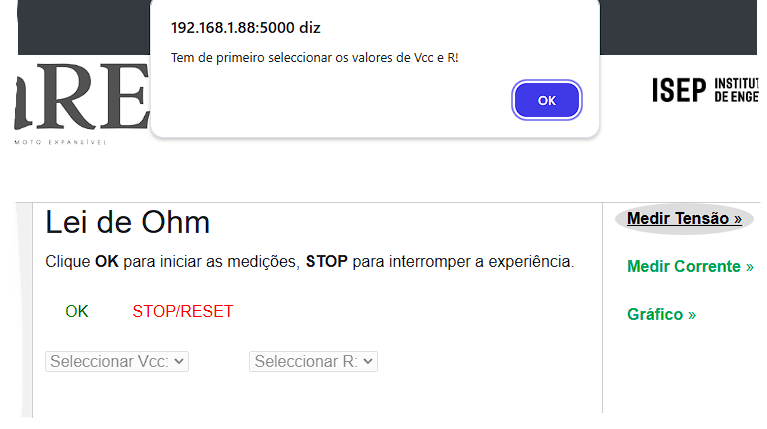
\includegraphics[width=0.7\textwidth]{figures/erro_pagina.png}
	\caption{Erro de selecção}
	\label{fig:erropagina}
\end{figure}

Como mencionado na Secção \ref{sec:frontend}, procurou-se manter a experiência de utilização e navegação o mais simples, prática e intuitiva possível. Além das páginas que compõem a base do \textit{site}, representadas na Figura \ref{fig:estruturapastas}, há ainda a juntar as que permitem ao utilizador interagir com as experiências do \acrshort{lare}. Especificamente, foram implementadas cinco páginas, correspondentes aos cinco circuitos definidos na Secção \ref{sec:solucaoproposta}.

A navegação ficou dividida da seguinte forma:
\begin{itemize}
	\item Autenticação;
	\begin{itemize}
		\item Página inicial;
		\begin{itemize}
			\item Página introdutória da experiência;
			\begin{itemize}
				\item Página de controle e realização da experiência.
			\end{itemize}
		\end{itemize}
	\end{itemize}
\end{itemize}

A página de autenticação, representada na Figura \ref{fig:paglogin}, está implementada no ficheiro \textit{auth.py}, função \textit{login}() e os formulários estão implementados na página \textit{login.html}, sendo que os dados de \textit{login} e registo são guardados na directoria \textit{instance}, ficheiro \textit{database.db}.

\begin{figure}[hbtp]
	\centering
	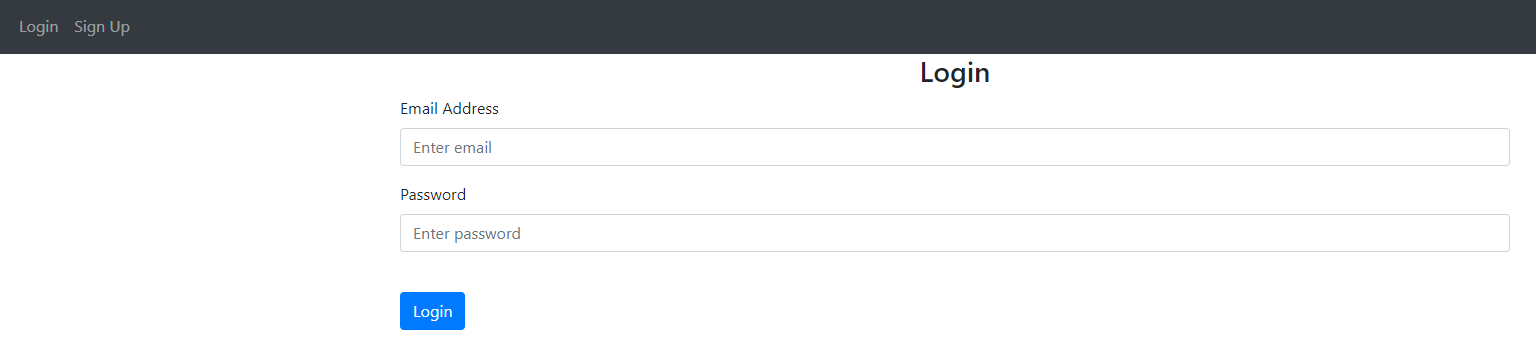
\includegraphics[width=0.3\textwidth]{figures/login.png}
	\caption{Página de \textit{login}}
	\label{fig:paglogin}
\end{figure}

%Além da rota definida para o \textit{login}, as outras rotas definidas no ficheiro \textit{auth.py} foram as \textit{sign-up} e \textit{logout}. A estrutura base da função \textit{login}, representada na Listagem \ref{lst:exemplologin}, é idêntica para as restantes, sendo que ``/\textit{login''} representa a rota especificada, dentro da função há o código especifico inerentes a cada função e o \textit{return render\_template} indica qual a página a ser renderizada.


%A título de exemplo, a página sobre a Lei de \textit{Ohm}, que é apresentada ao utilizador, está representada na Figura \ref{fig:ohm_intro}.

Após o registo e \textit{login} bem sucedido, é apresentada a página inicial, onde é feito um pequeno resumo do que é o \acrshort{lare} e apresentado o menu de escolha das experiências. O menu de separadores verticais foi retirado do \textit{site} \href{https://www.w3schools.com/howto/howto_js_vertical_tabs.asp}{\textit{W3Schools}} e modificado de acordo com as necessidades do projecto, tal como pode ser visto na Figura \ref{fig:pagmenu}.

\begin{figure}[hbtp]
	\centering
	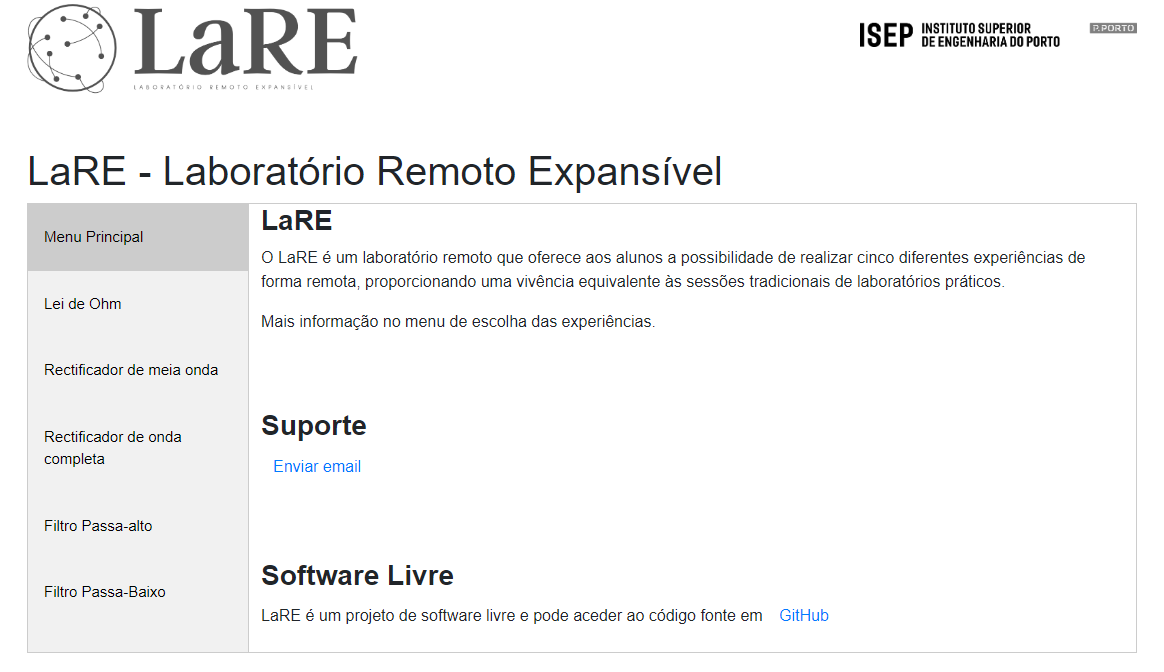
\includegraphics[width=0.7\textwidth]{figures/menupage.png}
	\caption{Página inicial}
	\label{fig:pagmenu}
\end{figure}

O modelo adoptado é uniforme para todas as experiências, apresentando o respectivo esquema e contextualização da actividade. Após a selecção da experiência, tanto as páginas introdutórias como as de controlo seguem a mesma estrutura de menus, mantendo o mesmo padrão de organização e navegação. A título de exemplo, as Figuras \ref{fig:ohm_intro} e \ref{fig:ohm_ctrl} ilustram, respetivamente, as páginas de introdução e controlo relativas à Lei de Ohm. 

% No entanto, no que diz respeito ao controlo das experiências, tal como referido na Secção \ref{sec:interfaceweb}, a experiência da Lei de \textit{Ohm} apresenta um maior grau de complexidade, dado que há um número maior de parâmetros e o utilizador ou aluno tem um controle mais amplo sobre a experiência.

\begin{figure}[hbtp]
	\centering%
		\centering
		\subfloat[\centering Introdução\label{fig:ohm_intro}]{{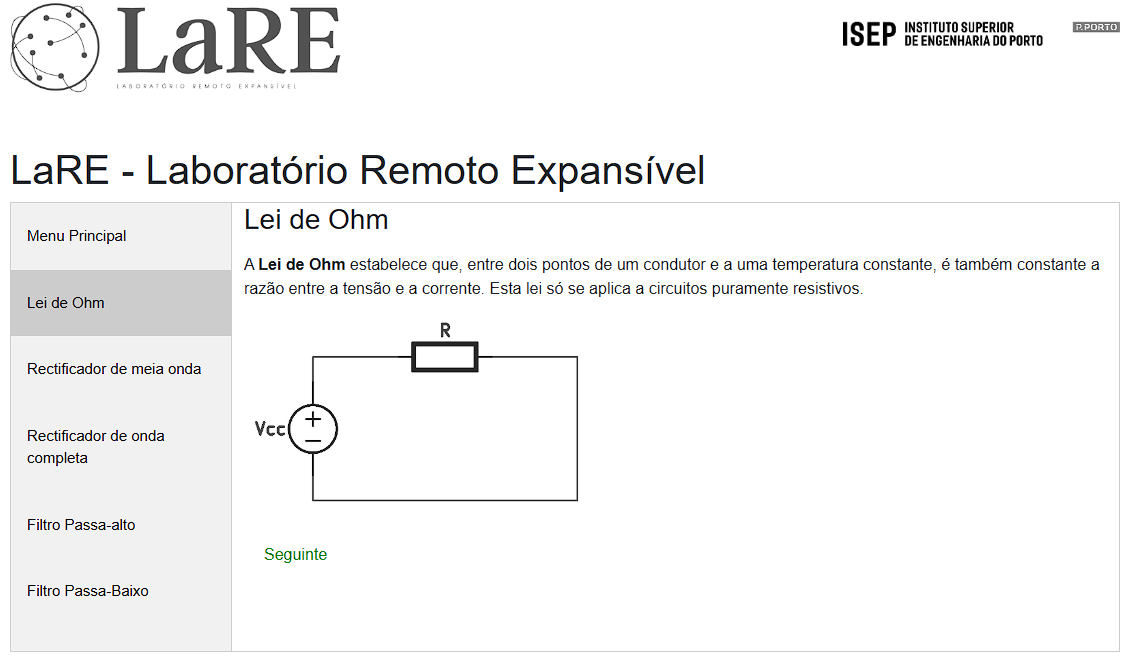
\includegraphics[width=6cm]{figures/ohm_page.png} }}%
		\qquad
		\subfloat[\centering Controlo\label{fig:ohm_ctrl}]{{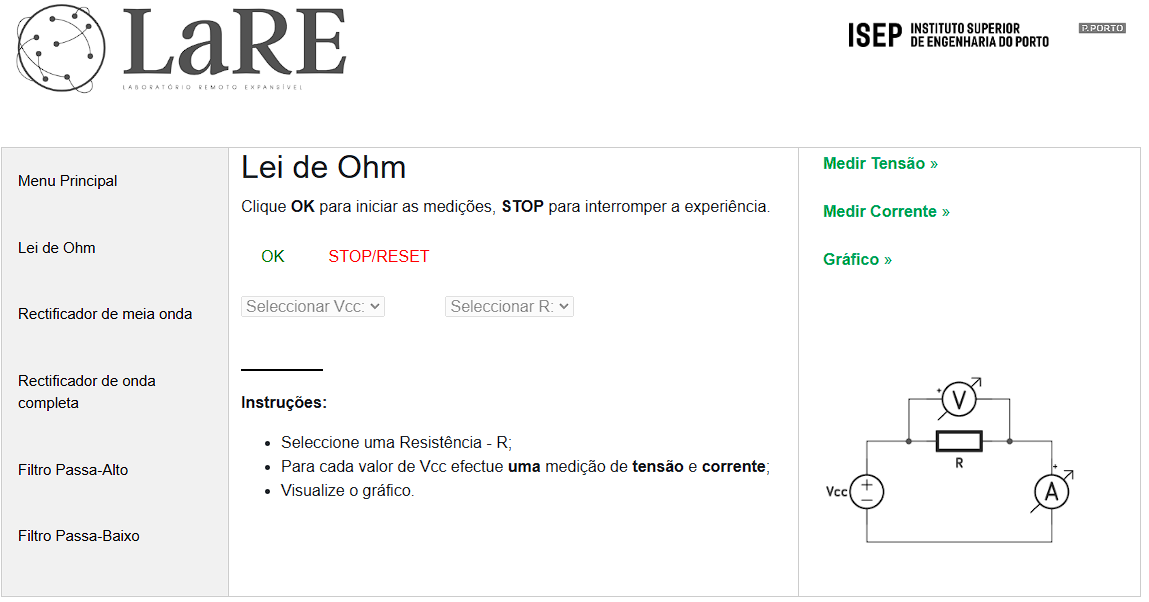
\includegraphics[width=6cm]{figures/ohm_page_controlo.png} }}%
		\caption{\textins{Exemplo} Experiência Lei de \textit{Ohm}}%
		\label{fig:pagohm}%
	\end{figure}

\subsubsection{Lei de \textit{Ohm}}
Nesta experiência, optou-se por conceder liberdade de escolha e controlo aos utilizadores, o que representou um desafio à implementação. Em vez de permitir apenas a selecção do valor da resistência, com medições realizadas (automaticamente) por \textit{software}, decidiu-se oferecer ao utilizador a possibilidade de escolher o valor da resistência e controlar as medições de tensão e corrente. Do ponto de vista pedagógico, considerou-se mais benéfico que, neste caso, os alunos verifiquem os valores das grandezas medidas à medida que realizam as medições e avançam na experiência. Além disso, o resultado e o gráfico final serão independentes da ordem pela qual se efectuam as medições.

A Figura \ref{fig:pagmenuCTRL} ilustra a página de controlo da experiência da Lei de \textit{Ohm}. 

\begin{figure}[hbtp]
	\centering
	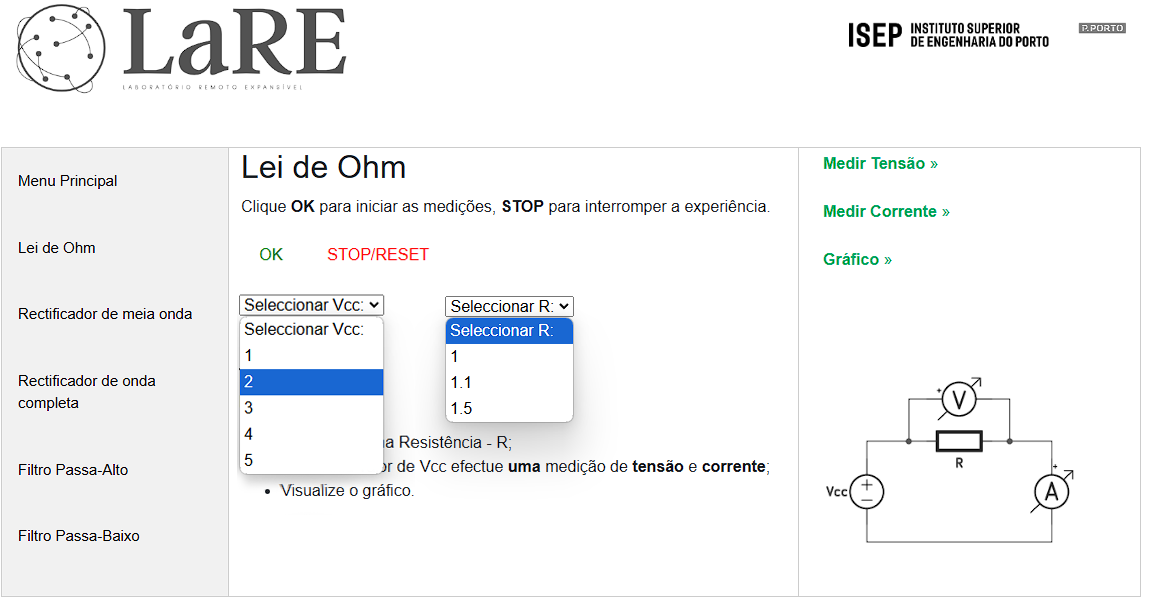
\includegraphics[width=0.7\textwidth]{figures/ohm_page_controlo-FULL.png}
	\caption{Lei de \textit{Ohm} - Selecção dos parâmetros}
	\label{fig:pagmenuCTRL}
\end{figure}

A selecção dos valores da resistência e do $U_{CC}$ \textbf{NOTA: Não esquecer de mudar o termo para Ucc nas páginas} é feita através de um formulário de selecção, feito em \acrshort{css} e \textit{JavaScript}, retirado do \textit{site} \href{https://www.w3schools.com/howto/howto_custom_select.asp}{\textit{W3Schools}} e modificado de acordo com as necessidades do projecto. Este formulário está implementado na página \acrshort{html} da experiência. Como se pode observar pela Figura \ref{fig:pagmenuCTRL}, embora a medição da tensão corresponda ao valor de $U_{CC}$ seleccionado, optou-se, por razões pedagógicas e de coerência com o esquema, por medir e apresentar a tensão aos terminais da resistência.

As medições só serão efectivamente realizadas e os valores apresentados, quando o utilizador seleccionar a opção ``Medir tensão'' e/ou ``Medir corrente''. 

Após a realização das dez medições, o utilizador pode seleccionar a opção ``Gráfico'' para visualizar o gráfico da experiência. (Se o gráfico for solicitado antes da conclusão de todas as medições, este será apresentado, embora de forma incompleta. No entanto, o utilizador poderá continuar a experiência sem impedimentos.

Sendo assim, o procedimento para a realização da experiência é o seguinte:
\begin{enumerate}
	\item Seleccionar ``OK'' para activar a fonte do \acrshort{virtualbench} e alimentar os integrados;
	\item Escolher o valor da resistência;
	\item Escolher o valor de $U_{CC}$;
	\item Efectuar cinco medições de tensão (``Medir tensão'') e cinco medições de corrente (``Medir corrente'');
	\item Ver o gráfico resultante.
	\item Seleccionar ``STOP/RESET'' para desactivar a fonte do \acrshort{virtualbench}.
\end{enumerate}

\subsubsection{Rectificador de meia onda e onda completa}
\label{sec:rectificadores}
Nestas duas experiências, pretende-se estudar e avaliar a diferença entre estes dois tipos de rectificadores, tanto ao nível da rectificação como da filtragem, nomeadamente no estudo da variação da tensão de \textit{ripple}.

A principal diferença, como foi referido na Secção \ref{sec:rectificadoresfiltros}, reside no valor da frequência. Enquanto que no rectificador de meia onda, o sinal de entrada é alimentado pelo gerador de sinal do \textit{virtualbench}, o rectificador de onda completa, devido ao problema de massa já referenciado na Secção \ref{sec:fontealternada}, é alimentado através de um transformador \SI{230}{\volt}/\SI{8}{\volt}, com uma frequência de \SI{50}{\hertz}.

A Figura \ref{fig:meiaondamenuCTRL} ilustra a página de controlo da experiência do rectificador de meia onda. Os utilizadores podem seleccionar quatro valores para o termo RC, sendo que os valores de C estão definidos para \SI{1}{\micro\farad} e \SI{10}{\micro\farad} e a frequência varia entre \SI{5}{\hertz} e \SI{2000}{\hertz}. 

\begin{figure}[hbtp]
	\centering%
		\centering
		\subfloat[\centering Rectificador de meia onda\label{fig:meiaondamenuCTRL}]{{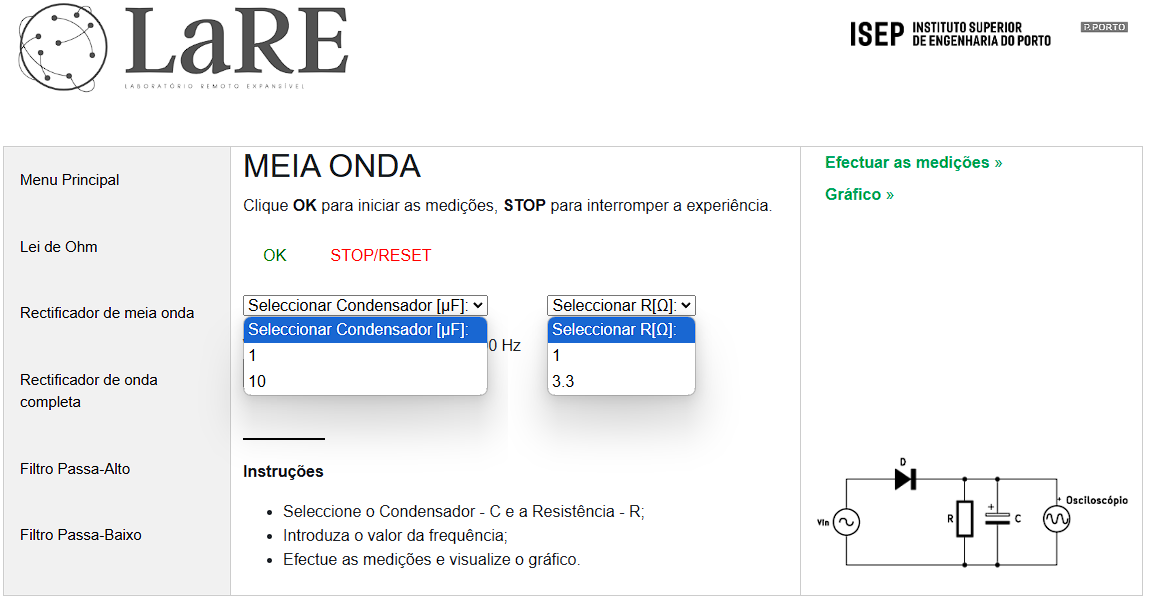
\includegraphics[width=6cm]{figures/meiaonda_page_controlo-FULL.png} }}%
		\qquad
		\subfloat[\centering Rectificador de onda completa\label{fig:ondacompletamenuCTRL}]{{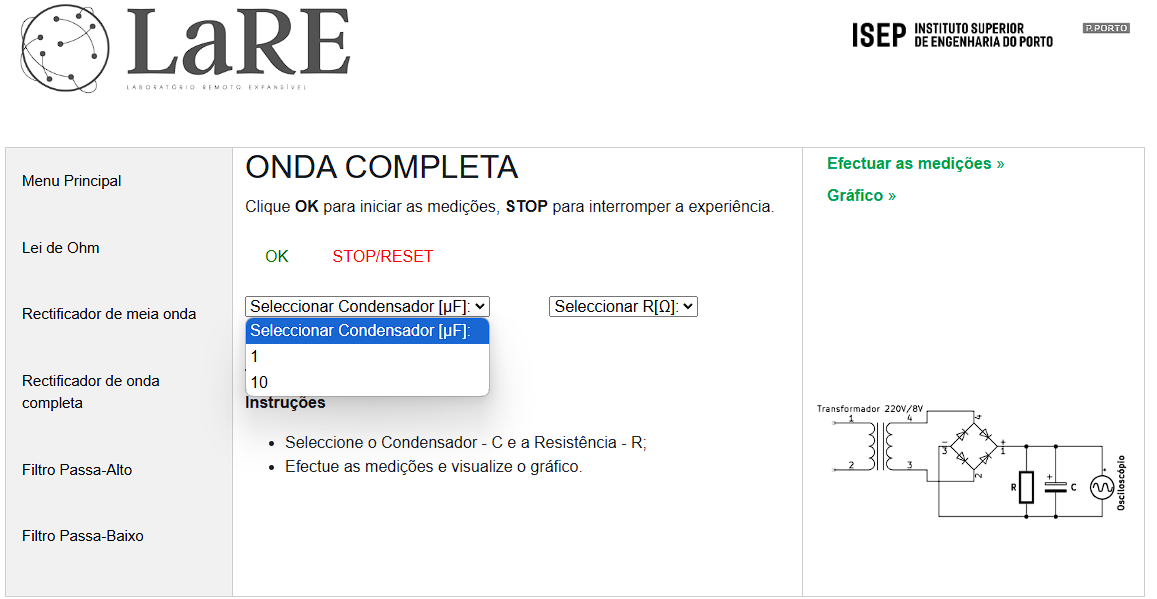
\includegraphics[width=6cm]{figures/ondacompleta_control.png} }}%
		\caption{Selecção de parâmetros}%
		\label{fig:seleccaoparametros}%
\end{figure}

As medições e construção do gráfico são realizadas por \textit{software}, baseadas nos valores seleccionados pelos utilizadores. Os resultados obtidos podem, então, ser comparados com o gráfico teórico, definido na Figura \ref{fig:sedraripple} ou pela Equação \ref{eq:vripple}. Para o mesmo par RC, os utilizadores podem, ainda, variar a frequência e comparar os resultados obtidos.

Relativamente ao rectificador de onda completa, a Figura \ref{fig:ondacompletamenuCTRL} apresenta a página de controlo da experiência, que é praticamente idêntica à do rectificador de meia onda, excepto pelo facto de a frequência não poder ser ajustada pelo utilizador. Os valores dos condensadores e resistências são os mesmos para ambas as experiências.

O procedimento para a realização da experiência é o seguinte:
\begin{enumerate}
	\item Seleccionar ``OK'' para activar a fonte do \acrshort{virtualbench} e alimentar os integrados;
	\item Escolher o valor da resistência;
	\item Escolher o valor do condensador;
	\item Efectuar as medições;
	\item Ver o gráfico resultante;
	\item Seleccionar ``STOP/RESET'' para desactivar a fonte do \acrshort{virtualbench}.
\end{enumerate}

\subsubsection{Filtros}
\label{sec:filtrosSW}
As páginas dos filtros passa-baixo e passa-alto, são em tudo idênticas às dos rectificadores e estão representadas na Figura \ref{fig:passabaixomenuCTRL} e Figura \ref{fig:passaaltomenuCTRL}. Os objectivos foram já definidos na Secção \ref{sec:objectivosexperiencias}.

\begin{figure}[hbtp]
	\centering%
		\centering
		\subfloat[\centering Filtro passa-baixo\label{fig:passabaixomenuCTRL}]{{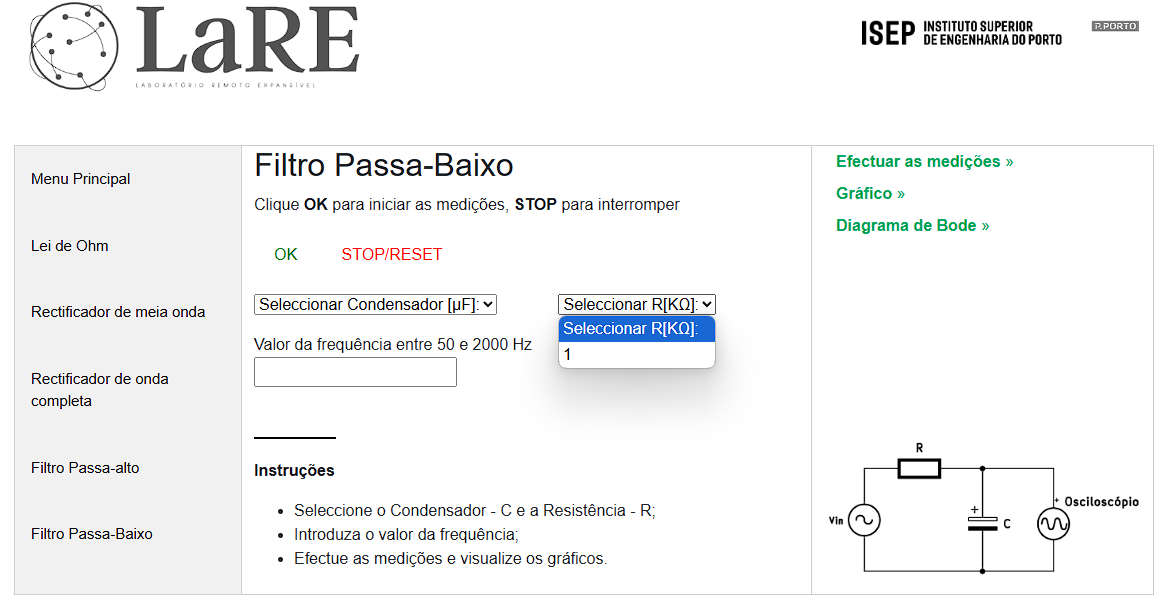
\includegraphics[width=6cm]{figures/passabaixo_page_controlo.png} }}%
		\qquad
		\subfloat[\centering Filtro passa-alto\label{fig:passaaltomenuCTRL}]{{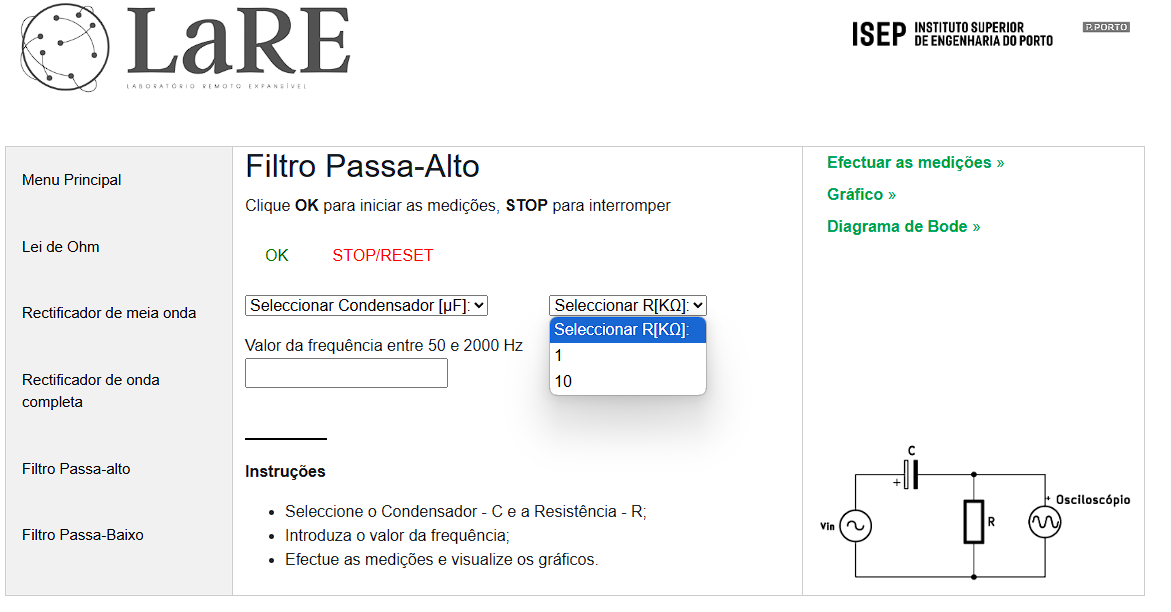
\includegraphics[width=6cm]{figures/passaalto_page_controlo.png} }}%
		\caption{Selecção de parâmetros}%
		\label{fig:controlofiltros}%
\end{figure}

Consoante a configuração do filtro, o utilizador escolhe entre dois condensadores ou duas resistências, representados no rectângulo tracejado cor-de-laranja, na Figura \ref{fig:rectificacao_filtragem_full}. Como já foi referido na Secção \ref{sec:experiencias}, os componentes dentro do rectângulo tracejado vermelho, representados na mesma figura, foram adicionados após a implementação dos rectificadores. Assim, quando se pretende estudar o filtro passa-baixo, o utilizador escolhe entre os dois condensadores (de saída) e se pretender estudar o passa-alto, escolhe entre as duas resistências (de saída). 

Eventualmente, poder-se-ia ter adicionado mais resistências/condensadores aos filtros, nomeadamente, no rectângulo tracejado vermelho, de forma a permitir uma maior versatilidade no estudo. No entanto, além de não existir o número suficiente de relés em contexto laboratorial, considerou-se que, desta forma, o estudo e os objectivos da experiência, ficariam provados. O intervalo de frequência mantém-se entre os \SI{50}{\hertz} e \SI{2000}{\hertz}. 

O procedimento para a realização da experiência é o seguinte:
\begin{enumerate}
	\item Seleccionar ``OK'' para activar a fonte do \acrshort{virtualbench} e alimentar os integrados;
	\item Escolher o valor do condensador - passa-baixo;
	\item Escolher o valor da resistência - passa-alto;
	\item Efectuar as medições;
	\item Ver o gráfico resultante;
	\item Ver o gráfico resultante da resposta em frequência;
	\item Seleccionar ``STOP/RESET'' para desactivar a fonte do \acrshort{virtualbench}.
\end{enumerate}